%============================================================================
% tento soubor pouzijte jako zaklad
% (c) 2008 Michal Bidlo
% E-mail: bidlom AT fit vutbr cz
%============================================================================
% kodovaní: UTF-8 (zmena prikazem iconv, recode nebo cstocs)
%----------------------------------------------------------------------------
% zpracování: make, make pdf, make clean
%============================================================================
% Šablonu upravil: Ing. Jaroslav Dytrych, idytrych@fit.vutbr.cz
%============================================================================
\documentclass[english]{fitthesis} % bez zadání - pro začátek práce, aby nebyl problém s překladem
%\documentclass[zadani]{fitthesis} % odevzdani do wisu - odkazy jsou barevné
%\documentclass[zadani,print]{fitthesis} % pro tisk - odkazy jsou černé
%\documentclass[english,print]{fitthesis} % pro tisk - odkazy jsou černé
% * Je-li prace psana v anglickem jazyce, je zapotrebi u tridy pouzit 
%   parametr english nasledovne:
%      \documentclass[english]{fitthesis}
% * Je-li prace psana ve slovenskem jazyce, je zapotrebi u tridy pouzit 
%   parametr slovak nasledovne:
%      \documentclass[slovak]{fitthesis}

\usepackage[czech,english]{babel}
\usepackage[utf8]{inputenc} %kodovani
\usepackage[T1]{fontenc}
\usepackage{cmap}
\usepackage{url}
\DeclareUrlCommand\url{\def\UrlLeft{<}\def\UrlRight{>} \urlstyle{tt}}

% zde muzeme vlozit vlastni balicky
\usepackage{listings}
\usepackage[toc,page,header]{appendix}
\RequirePackage{titletoc}
\ifczech
  \usepackage{ae}
\fi


%---rm---------------
\renewcommand{\rmdefault}{lmr}%zavede Latin Modern Roman jako rm
%---sf---------------
\renewcommand{\sfdefault}{qhv}%zavede TeX Gyre Heros jako sf
%---tt------------
\renewcommand{\ttdefault}{lmtt}% zavede Latin Modern tt jako tt

%-----------------------------------------------------------------------------


% Níže jsou deklarace fontů pro testování a ladění JVS 
% - doporučuje se NEPOUŽÍVAT
% Deklarace nejsou doladěné !!!
% Times New Roman není dle JVS povolený (je tu na ukázku)
%-----------------------------------------------------------------------------

\ifOPEN
  \pdfmapfile{=OpenSansfontspdf.map}
  \DeclareFontFamily{T1}{OpenSans}{}
  \DeclareFontShape{T1}{OpenSans}{b}{n}{<->recOpenSans-Bold}{}
  \DeclareFontShape{T1}{OpenSans}{b}{it}{<->recOpenSans-BoldItalic}{}
  \DeclareFontShape{T1}{OpenSans}{eb}{n}{<->recOpenSans-ExtraBold}{}
  \DeclareFontShape{T1}{OpenSans}{eb}{it}{<->recOpenSans-ExtraBoldItalic}{}
  \DeclareFontShape{T1}{OpenSans}{m}{it}{<->recOpenSans-Italic}{}
  \DeclareFontShape{T1}{OpenSans}{l}{n}{<->recOpenSans-Light}{}
  \DeclareFontShape{T1}{OpenSans}{l}{it}{<->recOpenSans-LightItalic}{}
  \DeclareFontShape{T1}{OpenSans}{m}{n}{<->recOpenSans-Regular}{}
  \DeclareFontShape{T1}{OpenSans}{sb}{n}{<->recOpenSans-Semibold}{}
  \DeclareFontShape{T1}{OpenSans}{sb}{it}{<->recOpenSans-SemiboldItalic}{}
  \renewcommand{\rmdefault}{OpenSans}
  \renewcommand{\sfdefault}{OpenSans}
\else
  \iftoggle{declare_open}{
    \pdfmapfile{=OpenSansfontspdf.map}
    \DeclareFontFamily{T1}{OpenSans}{}
    \DeclareFontShape{T1}{OpenSans}{b}{n}{<->recOpenSans-Bold}{}
    \DeclareFontShape{T1}{OpenSans}{b}{it}{<->recOpenSans-BoldItalic}{}
    \DeclareFontShape{T1}{OpenSans}{eb}{n}{<->recOpenSans-ExtraBold}{}
    \DeclareFontShape{T1}{OpenSans}{eb}{it}{<->recOpenSans-ExtraBoldItalic}{}
    \DeclareFontShape{T1}{OpenSans}{m}{it}{<->recOpenSans-Italic}{}
    \DeclareFontShape{T1}{OpenSans}{l}{n}{<->recOpenSans-Light}{}
    \DeclareFontShape{T1}{OpenSans}{l}{it}{<->recOpenSans-LightItalic}{}
    \DeclareFontShape{T1}{OpenSans}{m}{n}{<->recOpenSans-Regular}{}
    \DeclareFontShape{T1}{OpenSans}{sb}{n}{<->recOpenSans-Semibold}{}
    \DeclareFontShape{T1}{OpenSans}{sb}{it}{<->recOpenSans-SemiboldItalic}{}
  }
\fi


\ifVAFLE
  \pdfmapfile{=Vafle_VUT_fontspdf.map}
  \DeclareFontFamily{T1}{VafleVUT}{}
  \DeclareFontShape{T1}{VafleVUT}{m}{n}{<->recVafle_VUT_Regular}{}
  \DeclareFontShape{T1}{VafleVUT}{b}{n}{<->recVafle_VUT_Bold}{}
  \DeclareFontShape{T1}{VafleVUT}{l}{n}{<->recVafle_VUT_Light}{}
  \renewcommand{\rmdefault}{VafleVUT}
  \renewcommand{\sfdefault}{VafleVUT}
  % Tohle je škaredý hack - Vafle nemá it a když se s tím nic neudělá, kurzíva
  % se nijak neprojeví (jen varováním při překladu). Nicméně "doplňkový" font 
  % OpenSans kurzívu má a v semibold to dle mého názoru vypadá pro demonstrační
  % účely při ladění JVS přijatelně.
  \let\oldit\it
  \renewcommand{\it}{\usefont{T1}{OpenSans}{sb}{it}}
\else
  \ifTVAFLE
    \pdfmapfile{=Vafle_VUT_fontspdf.map}
    \DeclareFontFamily{T1}{VafleVUT}{}
    \DeclareFontShape{T1}{VafleVUT}{m}{n}{<->recVafle_VUT_Regular}{}
    \DeclareFontShape{T1}{VafleVUT}{b}{n}{<->recVafle_VUT_Bold}{}
    \DeclareFontShape{T1}{VafleVUT}{l}{n}{<->recVafle_VUT_Light}{}
    \pdfmapfile{=OpenSansfontspdf.map}
    \DeclareFontFamily{T1}{OpenSans}{}
    \DeclareFontShape{T1}{OpenSans}{b}{n}{<->recOpenSans-Bold}{}
    \DeclareFontShape{T1}{OpenSans}{b}{it}{<->recOpenSans-BoldItalic}{}
    \DeclareFontShape{T1}{OpenSans}{eb}{n}{<->recOpenSans-ExtraBold}{}
    \DeclareFontShape{T1}{OpenSans}{eb}{it}{<->recOpenSans-ExtraBoldItalic}{}
    \DeclareFontShape{T1}{OpenSans}{m}{it}{<->recOpenSans-Italic}{}
    \DeclareFontShape{T1}{OpenSans}{l}{n}{<->recOpenSans-Light}{}
    \DeclareFontShape{T1}{OpenSans}{l}{it}{<->recOpenSans-LightItalic}{}
    \DeclareFontShape{T1}{OpenSans}{m}{n}{<->recOpenSans-Regular}{}
    \DeclareFontShape{T1}{OpenSans}{sb}{n}{<->recOpenSans-Semibold}{}
    \DeclareFontShape{T1}{OpenSans}{sb}{it}{<->recOpenSans-SemiboldItalic}{}
  \fi
\fi

\ifARIAL
  \pdfmapfile{=arialfontspdf.map}
  \DeclareFontFamily{T1}{arial}{}
  \DeclareFontShape{T1}{arial}{b}{n}{<->recarialbd}{}
  \DeclareFontShape{T1}{arial}{b}{sl}{<->recarialbdo}{}
  \DeclareFontShape{T1}{arial}{b}{it}{<->recarialbi}{}
  \DeclareFontShape{T1}{arial}{m}{n}{<->recarial}{}
  \DeclareFontShape{T1}{arial}{m}{sl}{<->recarialo}{}
  \DeclareFontShape{T1}{arial}{m}{it}{<->recariali}{}
  \DeclareFontShape{T1}{arial}{bx}{n}{<->ssub * arial/b/n}{}
  \DeclareFontShape{T1}{arial}{bx}{sl}{<->ssub * arial/b/sl}{}
  \DeclareFontShape{T1}{arial}{bx}{it}{<->ssub * arial/b/it}{}
  \renewcommand{\rmdefault}{arial}
  \renewcommand{\sfdefault}{arial}
\else
  \ifTARIAL
    \pdfmapfile{=arialfontspdf.map}
    \DeclareFontFamily{T1}{arial}{}
    \DeclareFontShape{T1}{arial}{b}{n}{<->recarialbd}{}
    \DeclareFontShape{T1}{arial}{b}{sl}{<->recarialbdo}{}
    \DeclareFontShape{T1}{arial}{b}{it}{<->recarialbi}{}
    \DeclareFontShape{T1}{arial}{m}{n}{<->recarial}{}
    \DeclareFontShape{T1}{arial}{m}{sl}{<->recarialo}{}
    \DeclareFontShape{T1}{arial}{m}{it}{<->recariali}{}
    \DeclareFontShape{T1}{arial}{bx}{n}{<->ssub * arial/b/n}{}
    \DeclareFontShape{T1}{arial}{bx}{sl}{<->ssub * arial/b/sl}{}
    \DeclareFontShape{T1}{arial}{bx}{it}{<->ssub * arial/b/it}{}
  \fi
\fi

\ifTIMES
  \pdfmapfile{=timesfontspdf.map}
  \DeclareFontFamily{T1}{times}{}
  \DeclareFontShape{T1}{times}{m}{n}{<->rectimes}{}
  \DeclareFontShape{T1}{times}{m}{it}{<->rectimesi}{}
  \DeclareFontShape{T1}{times}{b}{n}{<->rectimesbd}{}
  \DeclareFontShape{T1}{times}{b}{it}{<->rectimesbi}{}
  \renewcommand{\rmdefault}{times}
  \renewcommand{\sfdefault}{times}
\fi


% moje
\usepackage{float}
\usepackage{mathtools}
\usepackage{amsmath, amsfonts}
\newcommand{\itab}[1]{\hspace{0em}\rlap{#1}}
\newcommand{\tab}[1]{\hspace{.22\textwidth}\rlap{#1}}
\newcommand{\quotes}[1]{``#1''}

\usepackage[dvipsnames]{xcolor}
\usepackage{pxfonts}

% style pro listing
\lstset{language=C++,
      basicstyle=\ttfamily,
      keywordstyle=\bfseries\color{Blue}\ttfamily,
      stringstyle=\color{YellowOrange}\ttfamily,
      commentstyle=\color{ForestGreen}\ttfamily,
      morecomment=[l][\color{Purple}]{\#}
}

% vypne funkci nové šablony, která automaticky nahrazuje uvozovky,
% aby nebyly prováděny nevhodné náhrady v popisech API apod.
\csdoublequotesoff

% =======================================================================
% balíček "hyperref" vytváří klikací odkazy v pdf, pokud tedy použijeme pdflatex
% problém je, že balíček hyperref musí být uveden jako poslední, takže nemůže
% být v šabloně
\ifWis
\ifx\pdfoutput\undefined % nejedeme pod pdflatexem
\else
  \usepackage{color}
  \usepackage[unicode,colorlinks,hyperindex,plainpages=false,pdftex]{hyperref}
  \definecolor{links}{rgb}{0.4,0.5,0}
  \definecolor{anchors}{rgb}{1,0,0}
  \def\AnchorColor{anchors}
  \def\LinkColor{links}
  \def\pdfBorderAttrs{/Border [0 0 0] }  % bez okrajů kolem odkazů
  \pdfcompresslevel=9
\fi
\else % pro tisk budou odkazy, na které se dá klikat, černé
\ifx\pdfoutput\undefined % nejedeme pod pdflatexem
\else
  \usepackage{color}
  \usepackage[unicode,colorlinks,hyperindex,plainpages=false,pdftex,urlcolor=black,linkcolor=black,citecolor=black]{hyperref}
  \definecolor{links}{rgb}{0,0,0}
  \definecolor{anchors}{rgb}{0,0,0}
  \def\AnchorColor{anchors}
  \def\LinkColor{links}
  \def\pdfBorderAttrs{/Border [0 0 0] } % bez okrajů kolem odkazů
  \pdfcompresslevel=9
\fi
\fi

%Informace o praci/projektu
%---------------------------------------------------------------------------
\projectinfo{
  %Prace
  project=BP,            %typ prace BP/SP/DP/DR
  year=2016,             %rok
  date=\today,           %datum odevzdani
  %Nazev prace
  title.cs={Sledování historie aktivity IP adres},  %nazev prace v cestine ci slovenstine (dle zadani)
  title.en={IP Address Activity Monitoring}, %nazev prace v anglictine
  %Autor
  author={Kateřina Pilátová},   %cele jmeno a prijmeni autora
  author.name={Kateřina},   %jmeno autora (pro citaci)
  author.surname={Pilátová},   %prijmeni autora (pro citaci)
  %author.title.p=Bc., %titul pred jmenem (nepovinne)
  %author.title.a=PhD, %titul za jmenem (nepovinne)
  %Ustav
  department=UPSY, % doplnte prislusnou zkratku dle ustavu na zadani: UPSY/UIFS/UITS/UPGM
  %Skolitel
  supervisor=Václav Bartoš, %cele jmeno a prijmeni skolitele
  supervisor.name={Václav},   %jmeno skolitele (pro citaci)
  supervisor.surname={Bartoš},   %prijmeni skolitele (pro citaci)
  supervisor.title.p=Ing.,   %titul pred jmenem (nepovinne)
  %supervisor.title.a={},    %titul za jmenem (nepovinne)
  %Klicova slova, abstrakty, prohlaseni a podekovani je mozne definovat 
  %bud pomoci nasledujicich parametru nebo pomoci vyhrazenych maker (viz dale)
  %===========================================================================
  %Klicova slova
  %keywords.cs={Klíčová slova v českém jazyce.}, %klicova slova v ceskem ci slovenskem jazyce
  %keywords.en={Klíčová slova v anglickém jazyce.}, %klicova slova v anglickem jazyce
  %Abstract
  %abstract.cs={Výtah (abstrakt) práce v českém jazyce.}, % abstrakt v ceskem ci slovenskem jazyce
  %abstract.en={Výtah (abstrakt) práce v anglickém jazyce.}, % abstrakt v anglickem jazyce
  %Prohlaseni
  %declaration={Prohlašuji, že jsem tuto bakalářskou práci vypracoval samostatně pod vedením pana ...},
  %Podekovani (nepovinne)
  %acknowledgment={Zde je možné uvést poděkování vedoucímu práce a těm, kteří poskytli odbornou pomoc.} % nepovinne
}

%Abstrakt (cesky, slovensky ci anglicky)
\abstract[cs]{Poslední dobou se objem přenášených dat po síti neustále zvyšuje.
K~urychlení prohledávání dat je potřeba mít způsob jejich vhodné indexace.
Tato bakalářská práce se zabývá tímto problémem, konkrétně ukládáním a~vyhledáváním
dat za účelem zjištění aktivity komunikujících IP adres. Cílem této práce je
navrhnout a~implementovat systém pro efektivní dlouhodobé ukládání a~vizualizaci aktivity IP adres.
Aktivitou je myšleno, zda daná adresa generovala provoz v~daném intervalu či ne,
tedy lze ji reprezentovat jediným bitem, což redukuje objem prohledávaných dat.
Výsledný systém se skládá z~backendu monitorujícího provoz a~ukládajícího
 záznamy o~aktivitě do uložiště a~jejich parametry do
konfiguračního souboru. Dále obsahuje webový server, který na základě požadavků
uživatele data čte a~vizualizuje ve formě obrázků. Uživatel může specifikovat
oblast dat, kterou chce zkoumat podrobněji, pomocí interaktivního webového rozhraní.}
\abstract[en]{The volume of generated network traffic continually grows.
In order to query data inside the traffic, an effective system of
indexing data is required. This thesis addresses this problem, specifically
effectively storing data for a~longer period of time and
looking up this data representing activity of communicating IP addresses.
The aim of this thesis is to design and implement a~system that stores
and visualizes IP address activity. Activity means whether given address
generated traffic during a~given interval or not. This information has
a~binary value and can be represented by one bit, which significantly reduces
volume of queried data. The system consists of backend processing incoming
flow records and storing address activity to binary storage. Furthermore, it
contains a~web server which reads stored activity and visualises it
in the form of an image based on user's request. The user can specify
an area they wish to examine in more detail in the interactive web interface.}

%Klicova slova (cesky, slovensky ci anglicky)
\keywords[cs]{monitorování sítě, aktivita IP adres, NEMEA, libtrap, IPFIX, analýza datových toků}
\keywords[en]{Network Monitoring, IP Address Activity, NEMEA, libtrap, IPFIX, Flow Analysis}

%Prohlaseni (u anglicky psane prace anglicky, u slovensky psane prace slovensky)
\declaration{Hereby I declare that this bachelor's thesis was prepared
as an original author’s work under the supervision of Ing. Václav Bartoš.
The supplementary information was provided by Ing. Tomáš Čejka.
All the relevant information sources, which were used during preparation
of this thesis, are properly cited and included in the list of references.}

%Podekovani (nepovinne, nejlepe v jazyce prace)
\acknowledgment{I wish to express my sincere thanks to my supervisor,
Ing. Václav Bartoš, for the guidance and encouragement. I am also grateful
to Ing. Tomáš Čejka, my consultant, for providing me with all the necessary
facilities, sharing expertise and guidance.}

\extendedabstract{
V~poslední době je internet běžnou součástí života a~objem
přenášených dat je čím dál tím větší. Aby se urychlilo vyhledávání dat,
je potřeba mít způsob, jak data vhodně indexovat. Jedním typem těchto dat jsou
IP adresy komunikujících zařízení. Tato bakalářská práce se tímto
problémem zabývá, konkrétně efektivním ukládáním a~vyhledáváním dat za účelem zjištění
aktivity komunikujících IP adres.

Cílem této bakalářské práce je navrhnout a~implementovat systém pro dlouhodobé ukládání a~vizualizaci
aktivity IP adres. Aktivitou adresy je myšleno, pokud adresa v daném časovém intervalu
generovala nějaký provoz či ne. Díky tomu, že má aktivita adres binární hodnotu, lze ji
efektivně uložit do binárního uložiště jako jediný bit. Takto se velikost uložiště a~objem
dat prohledaný při vyhledávání efektivně sníží.

Výsledný systém obsahuje backend, který analyzuje příchozí toky a~na konci každého intervalu
 ukládá záznamy o aktivitě adres patřících do zvoleného rozsahu do binárního uložiště.
Informace o parametrech uložiště jsou uchovávány ve speciálním konfiguračním souboru.
Dále obsahuje webový server, který pomocí konfiguračního souboru načte záznamy o~aktivitě
z~uložiště a~na základě požadavků uživatele ve webovém rozhraní vizualizuje tyto záznamy
a~pošle je webovému klientovi.

Uživatel si poté pomocí interaktivního webového rozhraní dostane informace o~záznamech a~může
zvolit konkrétní oblast ze zobrazované aktivity, kterou může zkoumat podrobněji.

V~kapitole \ref{sec:chapter2} jsou popsány principy monitorování a~NEMEA framework,
ve kterém je implementován backendový modul. Ve
\ref{sec:chapter3}. kapitole je detailněji popsán design výsledného systému a~použitých
technologií pro jednotlivé části. \ref{sec:chapter4}. kapitola je věnována popisu implementace
jednotlivých částí systému, detailnější vysvětlení nejdůležitějších jejich funkcí. Dále je
zde popis struktury a~určení míry efektivity binárního uložiště. Kapitola \ref{sec:chapter5}
je věnována popisu užitých technik testování a~jejich výsledků. V~kapitole \ref{sec:chapter6}
je vyhodnocení výsledků této bakalářské práce a~návrhy na možná další vylepšení tohoto projektu,
která budou realizována v~budoucnu.}

\begin{document}
  % Vysazeni titulnich stran
  % ----------------------------------------------
  \maketitle
  % Obsah
  % ----------------------------------------------
  \tableofcontents
  
  % Seznam obrazku a tabulek (pokud prace obsahuje velke mnozstvi obrazku, tak se to hodi)
\ifczech
  \renewcommand\listfigurename{Seznam obrázků}
\fi
\ifslovak
  \renewcommand\listfigurename{Zoznam obrázkov}
\fi

  % \listoffigures
\ifczech
  \renewcommand\listtablename{Seznam tabulek}
\fi
\ifslovak
  \renewcommand\listtablename{Zoznam tabuliek}
\fi

  % \listoftables 

  % Text prace
  % ----------------------------------------------
  %=========================================================================
% (c) Kateřina Pilátová, 3BIT
\setlength{\parindent}{0em}
\setlength{\parskip}{1em}

\csdoublequotesoff

\chapter{Introduction}\label{sec:chapter1}
Over the last decades, exchanging data over the Internet has become part of everyday life.
As the usage of networking became greater, the design of the networks became harder and so did securing network communication.
Network administrators monitor networks to maintain an overview of the network status, including used resources, users' activities or types of devices connected to the network.
Gathered data then helps administrators and designers make the network more suitable for their needs and increase the quality of the user experience. One of the collected parameters
are the IP addresses of the communicating endpoints, which is the main concern of this bachelor's thesis.

A~big volume of traffic is generated every day. Traffic consists of flow records carrying data between endpoints.
In order to make data lookup faster, a~special way of indexing data is required. The thesis addresses this problem and its purpose
is to make storing and querying activity of IP addresses more efficient.

The aim of this thesis is to design and implement a~system for storing and
visualising IP activity. The activity means whether traffic was
generated by/sent to a~given IP subnet in the monitored interval or not.
The resulting system consists of a~backend and a~frontend. The backend
is a NEMEA framework module that stores information about IP address activity
over a~longer period of time in binary storage and the data statistics to
a dedicated configuration file.
In order to reduce the lookup time, the activity of each subnet is represented by one bit.
Transforming stored data into images and providing information for the frontend is the~role of the web server.
The frontend, a~web client, visualises the final images and interacts with the user.
The user can then examine his areas of interest in more detail by
selecting an area in the whole image.

This thesis is divided as follows.
In Chapter~\ref{sec:chapter2}, network monitoring is discussed and the NEMEA framework is introduced as it is the used framework for the backend.
In Chapter~\ref{sec:chapter3}, attention is brought to the application design, which is described in detail and its aspects are evaluated.
In Chapter~\ref{sec:chapter4}, the components of the implemented module, backend, web server and graphical user interface, are defined and the essential sections and principles are explained.
Additionally, the structure the binary storage and its effectiveness is thoroughly discussed.
In Chapter~\ref{sec:chapter5}, testing methods of the module on both online and offline data are demonstrated and the results are examined
and any problems encountered and their solutions are discussed.
Chapter~\ref{sec:chapter6} is dedicated to a~discussion of the results, the
thesis summary and suggestions for possible improvements that could be added in the future.


% Network Monitoring in general
\chapter{Network Monitoring}\label{sec:chapter2}
The purpose of this chapter is to give the reader a~theoretical background to network monitoring and the framework used 
for implementing the module.
 
Network monitoring is a~part of network management that is used for maintaining the network status.
A~network monitoring system keeps track of devices and services based on traffic carried over the network.
An example of an engagement of such a~system can be seen in Figure~\ref{fig:monitoring}.

\begin{figure}[ht]
   \begin{center}
		\scalebox{0.4}{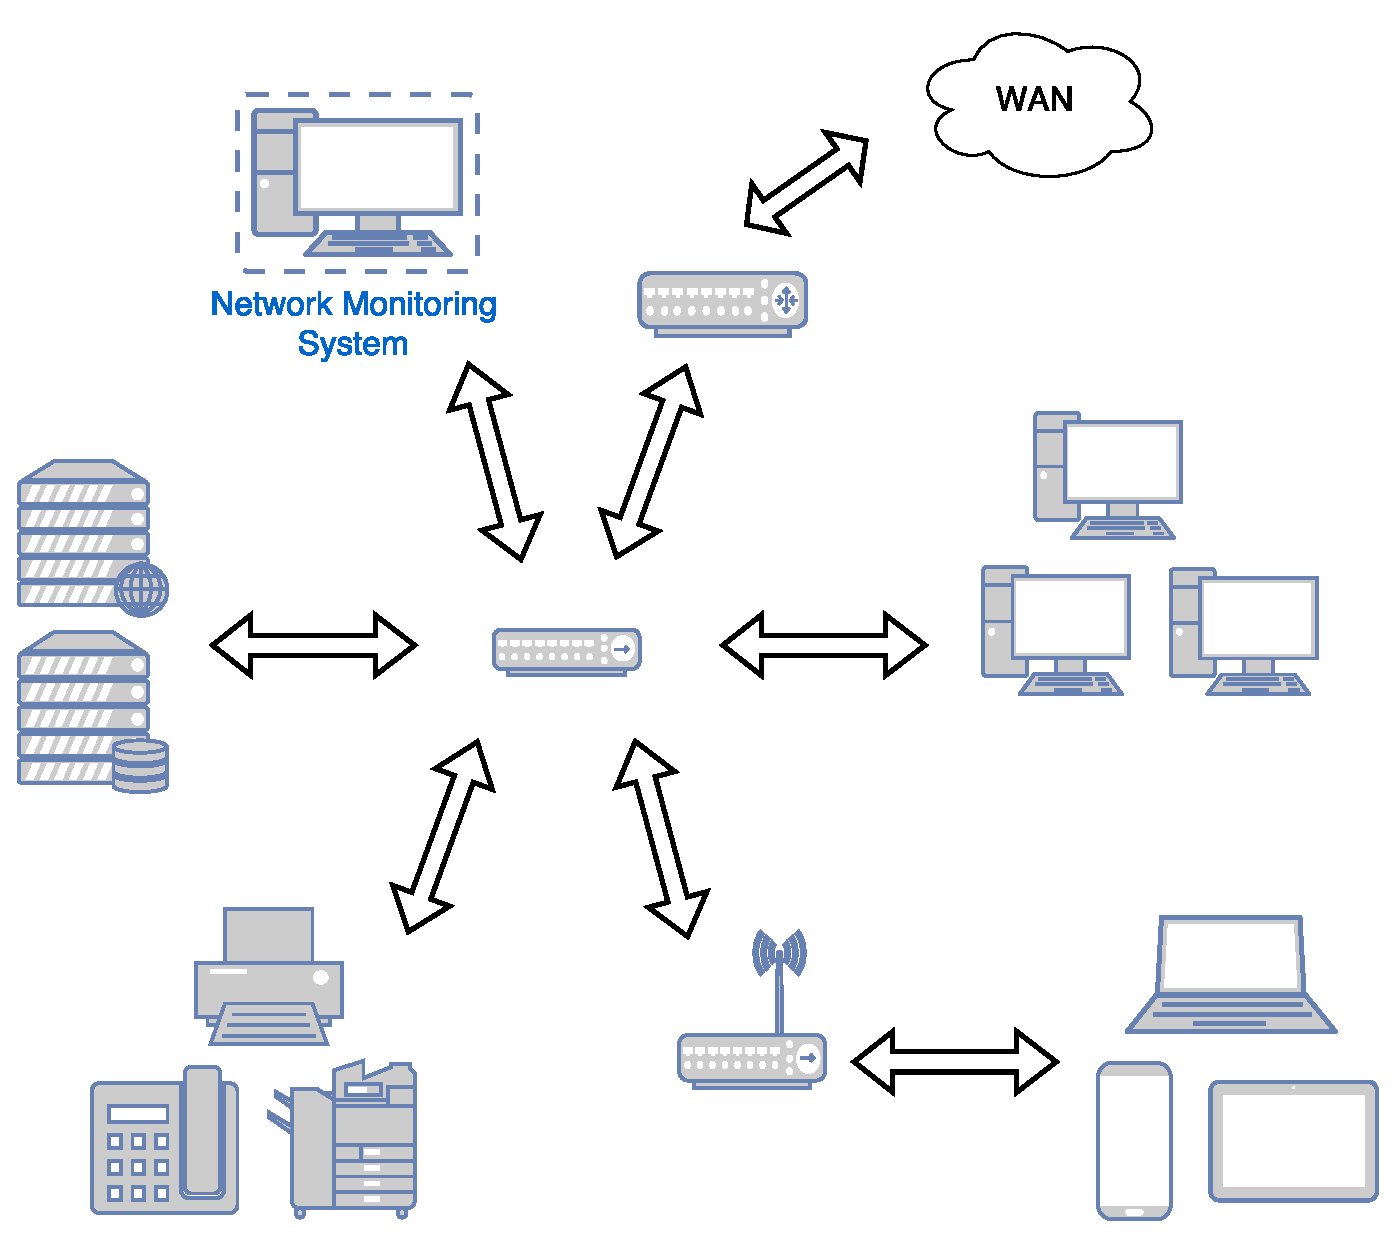
\includegraphics{fig/monitoring}} \hfill
      \caption{Example of monitored network containing Network Monitoring System} \label{fig:monitoring}
	\end{center}
\end{figure}

The target networks can be of different sizes (Local Area Network or Wide Area Network) and types (wired or wireless) and can consist of logically separated subnetworks. 

\section{The Purpose of Monitoring}
Network monitoring has many uses in various areas.
It can be used for detecting failing or malfunctioning components of the network that need to stay
running on various devices, such as servers, routers, desktops or switches. It also helps with cost saving by finding redundant resources or identifying
so-called \textit{bottlenecks}. Moreover, it can be used to improve performance by measuring
latency and spotting overloaded devices. Another example of monitoring usage is finding patterns that could signify security threats by analysing traffic.

\subsection{NfSen}\label{sec:nfsen}
An example of a~frontend for netflow~\cite{netflow} tools for storing and processing flow records called nfdump~\cite{nfdump} is NfSen~\cite{nfsen}.
It is an interface that displays how much data was transmitted over the probe in a~certain
time period. However, in order to find out the most active IP addresses, the user has to display the whole stored time interval.
To make the process faster and easier, the IP activity monitoring system can be used for displaying activity of the address space
in the whole time interval and for showing which addresses from the address space were active at
any the given moment. NfSen can then use the gained information to display how much traffic these addresses generated.

\section{Types of monitoring}
Monitoring can be either passive or active~\cite{isa_pa}. 
In active monitoring, the server continually polls for devices, applications and links status.
If a device does not respond in time, it is considered unavailable.
An example of a protocol used for active monitoring is the Internet Control Message Protocol (ICMP)~\cite{icmp}.
Passive monitoring only gathers information about the network that is carried over the listening port of the monitoring probe.
Information is sent in logs (for instance used in syslog~\cite{syslog}) or as data from network exporters
(like in the case of the IP Flow Information Export (IPFIX) protocol~\cite{ipfix}).

\section{Flow}
Nowadays, a~big volume of data is being transferred through the network. In order to make the processing and
transfer of captured traffic easier, monitoring systems are \textit{flow-based} --  probes firstly aggregate packets
into \textit{flows}~\cite{flow}.

A~flow is a set of IP packets passing an \textit{observation point} in the network during a~certain interval of time~\cite{ipfix}.
Packets that belong to the same flow share some properties in L3 (Network Layer), L4 (Transport Layer) or in some cases even
L7 (Application Layer) headers\footnote{Since the IP address is the only
attribute relevant to this thesis, the whole OSI model is not discussed in detail.}.
For instance, in the case of NetFlow, these parameters are the ingress
interface, source and destination IP address, source and destination port, IP protocol and Type of Service.

\section{Network Measurements Analysis (NEMEA) Framework}\label{sec:nemea}
% https://github.com/CESNET/ipfixcol/tree/master/plugins/storage/unirec
In this bachelor's thesis, the implemented module can be used in a~system called NEMEA.

NEMEA is a~modular system that allows for the custom analysis of traffic gathered both on-line and off-line.
Besides the Network and Transport Layer, of OSI Model analysis, it also enables the
examination of Application Layer (L7) data.

NEMEA processes data \textit{stream-wise} -- data arrives as individual records, one by one, unless it is explicitly defined otherwise.
Incoming records are analysed by the system without being stored aside along the way\footnote{The only case of storing incoming data is when it is
the~purpose of the particular participating module.}.

\subsection{Architecture}
An example of a~monitoring system architecture using NEMEA can be seen in Figure~\ref{fig:nemea_arch}:

\begin{figure}[ht]
   \begin{center}
		\scalebox{0.6}{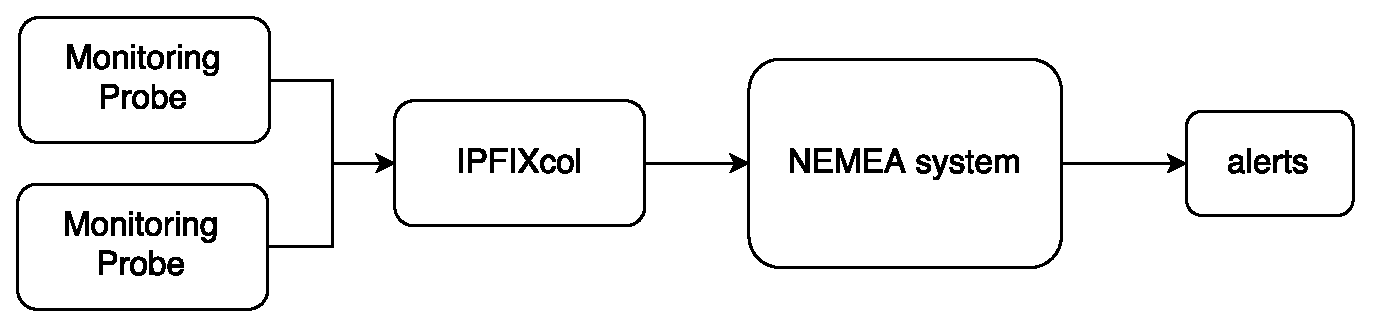
\includegraphics{fig/nemea_arch}} \hfill
      \caption{Architecture of Monitoring system including NEMEA} \label{fig:nemea_arch}
	\end{center}
\end{figure}

The system works as follows. The network is being monitored by monitoring probes (flow exporters).
Probes aggregate packets using IPFIX~\cite{ipfix} or NetFlow~\cite{netflow} technology and
export flows to a~central collector called IPFIXcol~\cite{ipfixcol}. The collector converts received
flows into another format called the Unified Record (UniRec)~\cite{ipfixcol} (explained
in section~\ref{sec:unirec}) and sends final flows to NEMEA.

NEMEA consists of modules that are assembled according to user's needs.
Each module can have multiple ingress and egress one-way TRAP (further discussed in
section~\ref{sec:libtrap}) interfaces~\cite{NEMEA_article}.
An example of a~set of interconnected modules is in Figure~\ref{fig:modules}
where \textit{Module 1} has two egress interfaces
that are connected to the only \textit{Module 2} and \textit{Module 3} ingress interface.

\begin{figure}[H]
   \begin{center}
		\scalebox{0.6}{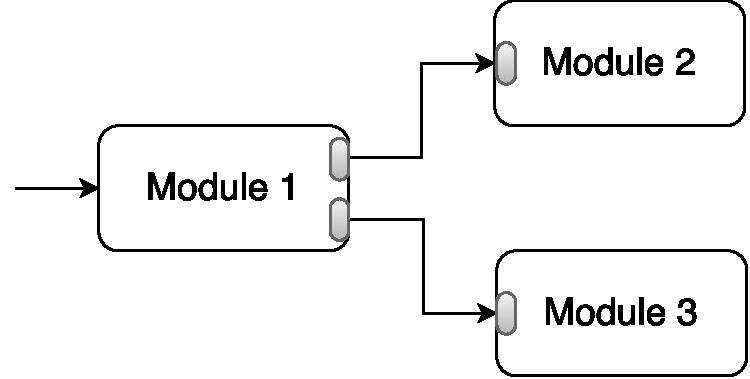
\includegraphics{fig/modules}} \hfill
      \caption{Interconnected modules} \label{fig:modules}.
	\end{center}
\end{figure}


Modules can be implemented in C or C++ and a~wrapper for Python is available.
The aim of this bachelor's thesis is to implement one such module.

\subsection{UniRec}\label{sec:unirec}
The UniRec format supports flow extension by Application Layer data and as a~result, makes accessing data in this layer easier.
The structure of this format can be seen in Figure~\ref{fig:unirec}.

\begin{figure}[H]
   \begin{center}
		\scalebox{0.6}{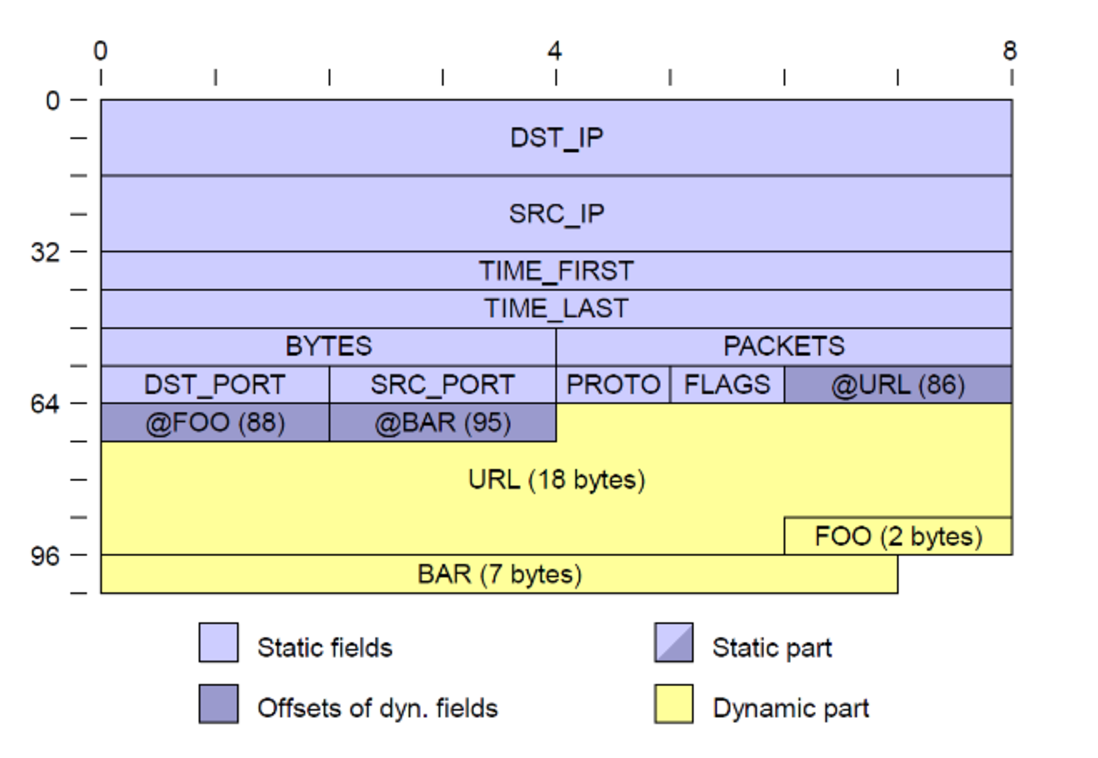
\includegraphics{fig/unirec}} \hfill
      \caption{UniRec Format} \label{fig:unirec}.
	\end{center}
\end{figure}

UniRec defines offsets for accessing fields in
various application layer protocols. Due to the diversity in the data sizes of individual protocols, this part
of the structure changes dynamically to correspond to the used protocol.

\subsection{Libtrap}\label{sec:libtrap}

TRAP is a~library (also called \textit{Libtrap}~\cite{libtrap}) that implements
common communication interfaces (IFC) used for communication among all NEMEA modules
as seen in Figure~\ref{fig:libtrap}. Communication is realised using either
TCP sockets (TCP/IP IFC) or Unix sockets (UNIX IFC).


\begin{figure}[H]
   \begin{center}
		\scalebox{0.6}{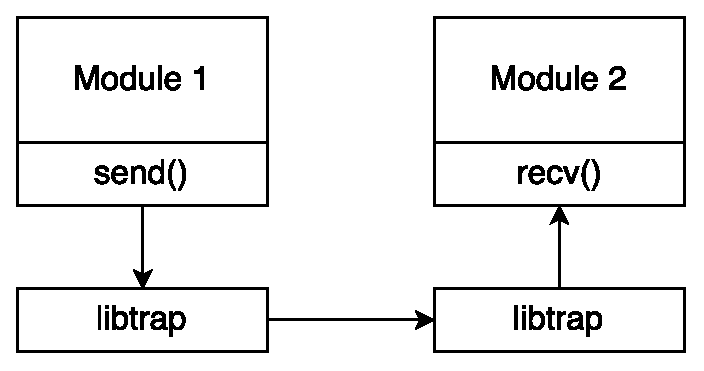
\includegraphics{fig/libtrap_communication}} \hfill
      \caption{NEMEA inter-module communication} \label{fig:libtrap}.
	\end{center}
\end{figure}

Libtrap contains features for controlling the communication and abstracts modules
from the complexity of the underlying interfaces.

\section{Related Work}
The method of visualizing traffic in the form of an image is quite common. Quite a~few projects are focused on
providing graphic information about communication on the network. One of the similar projects is
called \textit{Interactive Visualisation for Network and Port Scan Detection}~\cite{related}.

This project does not only examine IP activity but also includes port activity. This approach
does include more information about the monitored flows and offers more ways of visualising
the stored data but the size of the stored data is increased by the additional information
which leads to a~slower lookup time. This thesis is focused solely on one
attribute that can be used in other networking tools (for example NfSen~\ref{sec:nfsen}) as a~key for looking up
the rest of the data, including but not limited to the above-mentioned ports.

\csdoublequotesoff

% Design
\chapter{Application Design}\label{sec:chapter3}
This chapter discusses the design of the resulting system for visualizing IP address activity.
It introduces all system components and their functions, discusses technologies used for
realizing the system and suggests two main modes in which the system can be run.

\section{System Architecture}

\begin{figure}[ht]
   \begin{center}
		\scalebox{0.38}{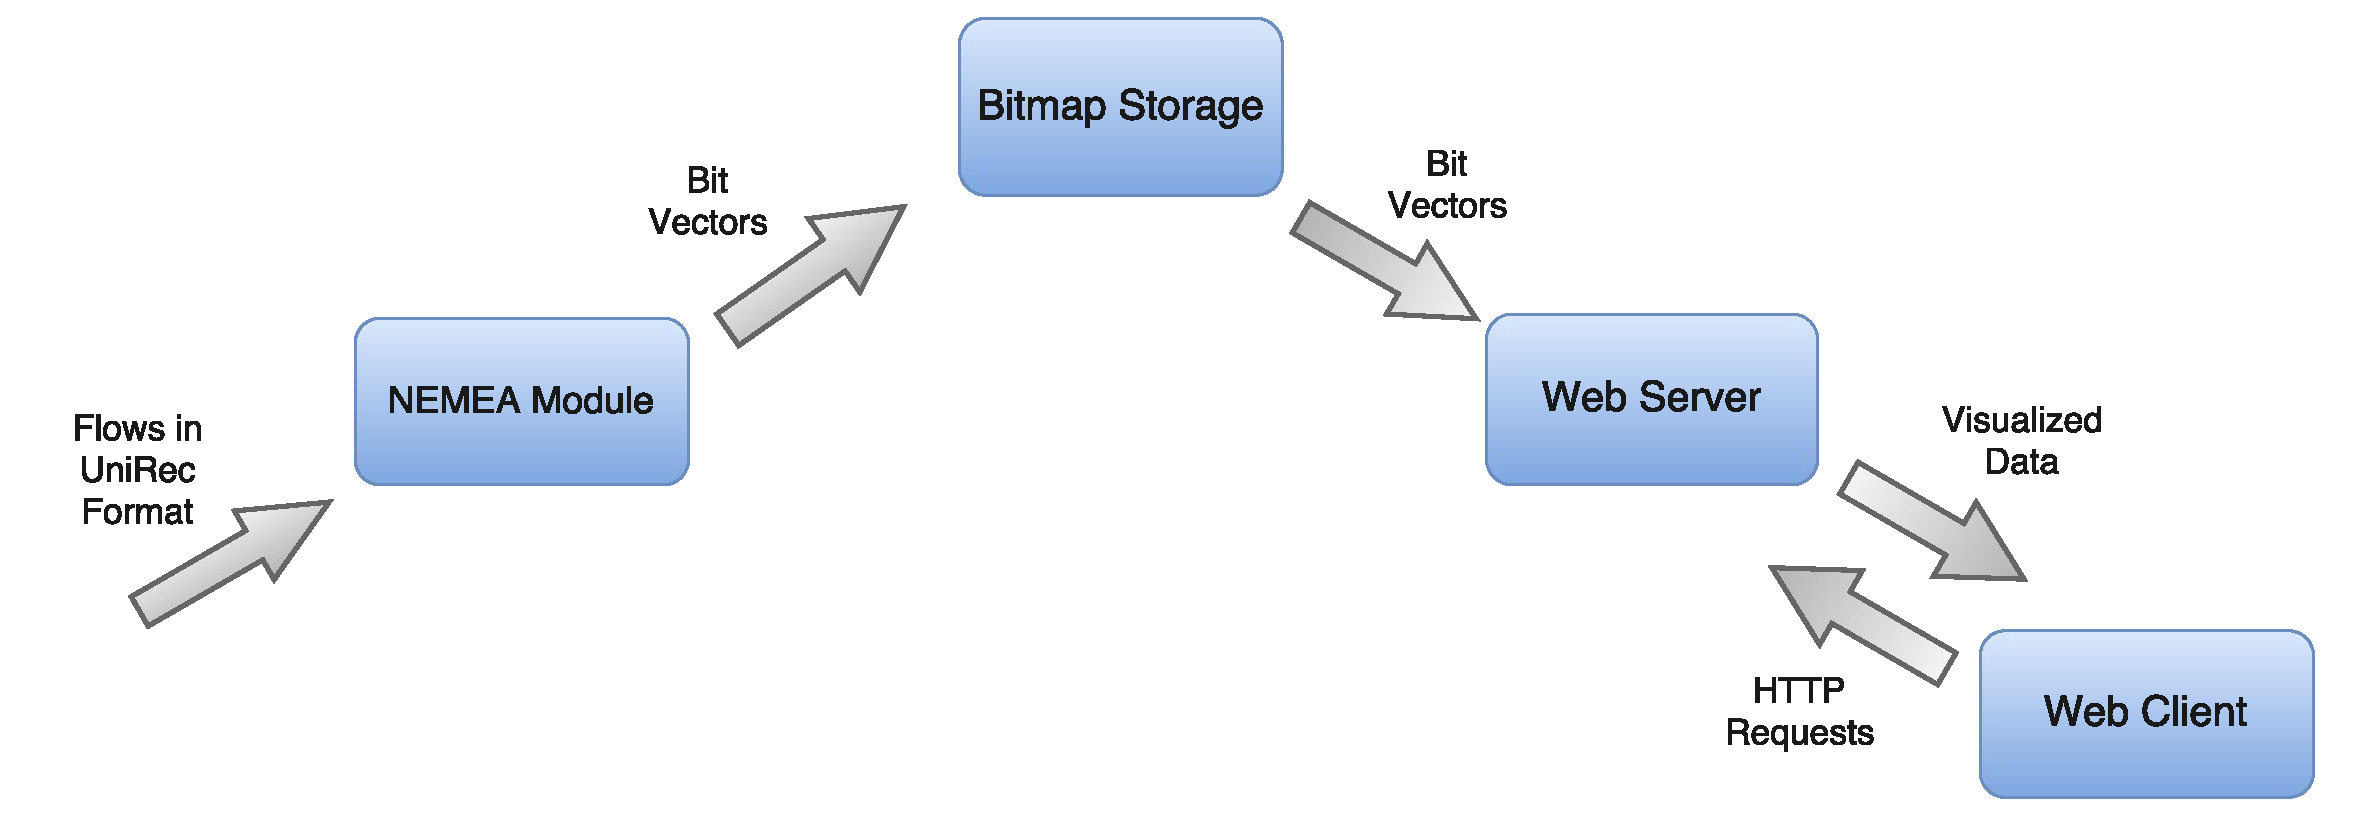
\includegraphics{fig/design}} \hfill
      \caption{System Design} \label{fig:design}
	\end{center}
\end{figure}

The system is illustrated in Figure~\ref{fig:design}. It consists of a NEMEA module, bitmap storage and
a web client and server. The Figure~\ref{fig:design} also shows the forms of data
transmitted between individual components or method for.

The module processes received data and saves it to the bitmap storage, represented by a~binary file.
The web client sends a request for visualisation of IP Activity to the server. The web server receives the request, retrieves data
from the storage based on inserted parameters and sends them back to the client. The web server runs independently of the module,
so that at any given moment, the configuration file must be up to date with the bitmap file state.

\section{Input and Output Data}
The main components ensuring the functionality of the system are the NEMEA module processing flows and the web server
providing visualisation to a~web client.
In this section, their possible inputs and outputs illustrated in Figure~\ref{fig:design} are discussed.

\subsection{NEMEA module}
For the NEMEA module, the input always consists of serialised flows that are received on its input interface in UniRec format.
The input data can be retrieved either directly from online traffic flowing through the probe or offline data generated from a~file.
The output of the module is a~bit vector representing activity of specified addresses (subnets) in a~given period of time and
it is written to a~dedicated binary file, followed by updating the configuration file.

\subsection{Web server}
The web server listens on a~predefined port and waits for requests from the client.
The HTTP requests may vary but they typically consist of a~URI containing several parameters that affect the server response.
The response of the server is requested information in form of a~response header value or an~image
(created from bitmap, see section~\ref{sec:bitmap}) reflecting the IP activity and
is sent back to the client.

\subsection{Web Client}\label{sec:client_design}
The client displays activity statistics and characteristics to the user. All the
displayed data is received from the server based on client's requests. 

\subsubsection{The Expected Users}
The group of users that are likely to interact with the interface is
expected to be familiar with the principles of networking and the NEMEA framework.
Therefore, this interface does not need any extended user guide, so the only
instructions describing the usage can be found at the About
section in the main menu.

The likely user scenarios are as follows:

\begin{itemize}
   \item User seeks to discover which IP subnets were active at a~particular time.
         The user provides the system with a~file containing recods from the desired time window.
   \item User wants to discover at which times the specified address space is/was active.
   \item User wants to examine an IP subnet or time interval activity more closely. They start the system
         multiple times with continually decreasing subnet/interval size to find out more detailed information.
\end{itemize}

By gaining the information about the IP activity, the user use this information to
examine the activity in other ways using tools such as NfSen (described in Section~\ref{sec:nfsen}).

\subsubsection{Layout}
The frontend layout is intended to be simple and readable for the user so that they are not
distracted or slowed down when interacting with the web interface. Used colour
combination has enough contrast to be easily readable. 
Selected options are displayed differently for better orientation.

The image colouring is selected in such a~way that the active areas stand out --
active places are displayed as white and inactive places as black. Undefined
areas have a~gray colour. The undefined value is used when the currently monitored
activity has a~lower interval range than the time window or when displaying
a~selected area. By doing so, the image proportions stay the same
(time window x number of subnets in the address space). The size of the image can be
changed by selecting a~ratio.

In order to avoid mixing up values from the background, the image is sorrounded
by a frame of a different colour.

Design of the layout structure is shown in Figure~\ref{fig:layout}.
\begin{figure}[ht]
   \begin{center}
		\scalebox{0.5}{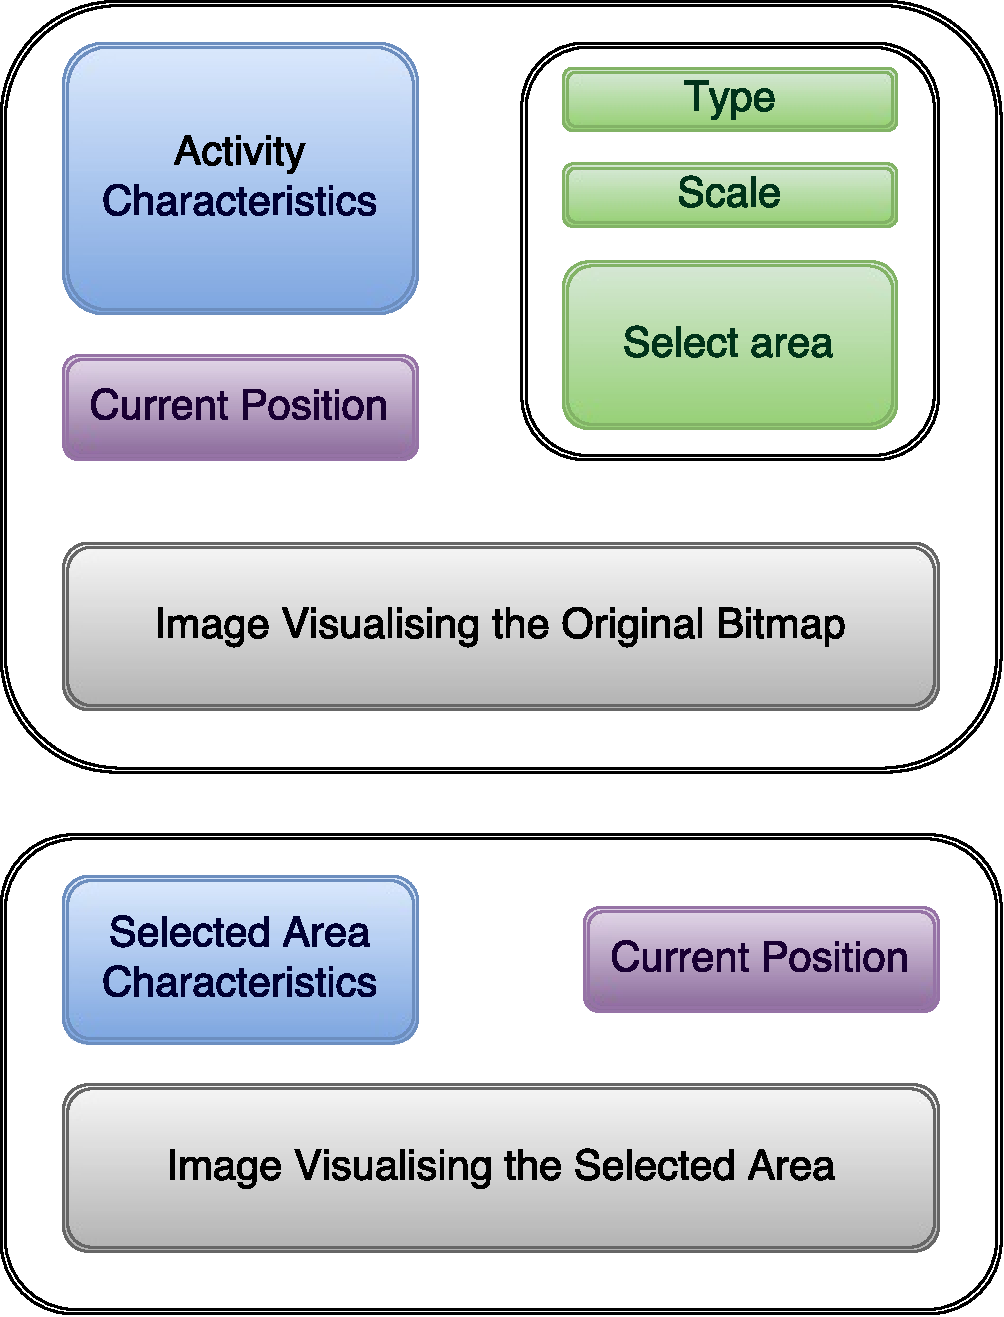
\includegraphics{fig/layout}} \hfill
      \caption{Frontend Layout} \label{fig:layout}
	\end{center}
\end{figure}

In the layout, the top part is dedicated to the original monitored area and
visualises the whole bitmap. The bottom part is hidden until the user selects
an area. All the Options are situated in the same section
(displayed as green coloured). The user can change the type of the original
bitmap and its scale at any time. In addition to this, they can also select
an area by inserting minimum and maximum values of the individividual axes.

Only after submitting the specified area, the bottom section is displayed.
Like in the top section, the area characteristics and current position are available
to the user, followed by the visualisation of the selected area.

The \textit{Current Position} section offers the user the ability to see the values of
the coordinates their cursor is pointing at. It is available for both the
original image and the selected area. The background of the \textit{Current Position}
field is adapted to the colour of currently visited subnet activity at a~particular moment.
Both subnet and time interval are displayed below the field title. 

\section{Result format}\label{sec:bitmap}
The result of the visualisation process is an~image, or a~set of images,
that represent IP address activity of communicating endpoints.
In order to cover all usage possibilities, separate images showing activity of monitored source IP addresses,
destination IP addresses and monitored links (source and destination pairs) are provided to the user.

An example of such image can be seen in Figure \ref{fig:image_example}. This
image is a~result of visualising activity at the nemea collector.
For better readability, the image was captured in scaling \texttt{2:1}. It contains
an undefined area (gray coloured) as the time window is not filled with activity record yet.

\begin{figure}[H]
   \begin{center}
		\scalebox{0.7}{\frame{
\includegraphics{fig/image_example}}} \hfill
      \caption{Visualised Activity} \label{fig:image_example}
	\end{center}
\end{figure}

The \textit{x}-axis represents time divided into defined units.
The \textit{y}-axis represents the range of predefined IP addresses to be
monitored. The principle of displaying measured activity can be defined as follows:

\begin{equation}\label{eq:image}
   \begin{multlined}
   \mbox{for }i \in \langle addr_{min}, addr_{max}\rangle, j \in \langle t_{min}, t_{max} \rangle: \\
   \quad x_{ij} = (1)_2 \Leftrightarrow \mbox{address } x_i \mbox{is active in time interval } j \\
   \quad x_{ij} = (0)_2 \Leftrightarrow \mbox{address } x_i \mbox{is inactive in time interval } j
   \end{multlined} 
\end{equation}

% Used Technologies
\section{Used Technologies}
\subsection {NEMEA Module}
For implementing the NEMEA module, languages Python, C or C++ can be used.

When using Python, the level of abstraction is greater and so the programmer
does not have an absolute control on how which abstract construction will be executed.
As a~result, the final module tends to be significantly slower due to unoptimised processing of
a~big volume of data in real time\footnote{This statement is based on earlier experience. When comparing
execution of the same functionality written in C and in Python, the module in Python was ten times slower.}.

C++ offers more options and functionalities than C, including a~special data structures for manipulation with bits
(such as \texttt{std::vector<bool>} or \texttt{std::bitset<size>}).
Furthermore, handling configuration file in YAML format is easier thanks to
\textit{YAML-cpp}~\cite{yaml_cpp} parser and emitter\footnote{The version of the package
must be \textit{0.5.3} which requires C++11 or \textit{Boost}~\cite{cppboost} libraries installed.}.
Therefore, the C++ language is used for the implementation.

For communication with the module, \textit{libtrap}~\cite{libtrap} is used.
Manipulating the received data is realised using \textit{UniRec} format.
These technologies are discussed in detail in section~\ref{sec:nemea}. 

\subsection{Web Server}\label{sec:python_packages}
PHP is mostly used as a~server-side programming language
for its universal usability and provided functions, e.g. communication with an SQL database.
However, in this architecture, the bitmap storage is represented by a~single binary file.

In the case of an SQL database, additional operations for connecting, retrieving
and processing data from the database in the form of tables are needed.
If heterogenous data are used, that can be an advantage. But in this system,
the only types of data needed are the information about the specified ranges
can easily be maintained in a~dedicated configuration file, and the binary data itself. 

Therefore, C++ or Python, each of which have their own libraries (or packages)
needed for a web server, can be used to realise needed functionality.

Due to a~convenient package called \textit{BaseHTTPServer}~\cite{httpserver}
(\textit{http.server} in Python 3) that manages HTTP functionality, the resulting
web server is implemented in Python. The implementation is compatible with
both 2.x and 3.x versions. For convenient work with various data types, the following non-standard packages are used:

\begin{itemize}
\item \itab{\footnotesize{\textit{beautifulsoup4}~\cite{beautifulsoup}}} \tab{Used for parsing and modifying HTML files.}
\item \itab{\footnotesize{\textit{bitarray}~\cite{beautifulsoup}}} \tab{Used for handling bit vectors.}
\item \itab{\footnotesize{\textit{ipaddress}~\cite{ipaddress}}} \tab{Package for convenient work with IP addresses.}
\item \itab{\footnotesize{\textit{Pillow}~\cite{pillow}}} \tab{The fork of \textit{PIL} (Python Imaging Library) for work with images.}
\item \itab{\footnotesize{\textit{pyyaml}~\cite{pyyaml}}} \tab{Parses YAML files (used for work with the configuration file).}
\end{itemize}

\subsection{Web Client}
When implementing a~web client, traditional web technologies are used:

\begin{itemize}
  \item \textit{HTML} -- defines the content of the web page
  \item \textit{CSS} -- specifies the layout of the web page
  \item \textit{JavaScript} -- describes the behaviour of the webpage, is often used asynchronously (\textit{AJAX})
\end{itemize}

The web client will use these technologies to achieve a well arranged graphical interface that
visualises data for the user and enables the user to specify an area that
is to be cropped from the original image and displayed separately.
Thanks to AJAX, all requests are handled asynchronously and no page reload
is needed in order to retrieve requested data.
In order to access and modify elements easily, JavaScript library \textit{jQuery}~\cite{jquery} is used.


\subsection{Conversion of a~bitmap to an image}
The web server uses a special module for visualising the bitmap (more in
section~\ref{sec:visualisation_handler}). This module uses a package for
processing images called Pillow~\cite{pillow} derived from \textit{Python Imaging Library}~\cite{pil}.

\csdoublequotesoff

% Implementation
\chapter{Implementation}\label{sec:chapter4}

% Backend
\section{Backend}
Backend is implemented in a~source file \texttt{ip\_activity.cpp}. In this part of the thesis,
operations carried on in this source file and associated data structures are discussed.

Backend receives parameters about the final image from the user,
and saves parameters to the configuration file, so that the server can index the stored data.
The program then scans incoming flow records and stores activity of defined address space in
each interval into the binary storage.

The \texttt{ip\_activity.cpp} module works with a~template containing at least three fields of
the UniRec format -- \texttt{SRC\_IP} (source IP address), \texttt{DST\_IP} (destination IP address)
and \texttt{TIME\_FIRST} (first occurrence of the flow).

In order to work properly, the module has to have writing privileges to the current folder where
the storage files and configuration file are to be created or rewritten.

\subsection{Workflow}
The workflow of the backend module is demonstrated in the Figure~\ref{fig:backend}.
It captures the main operations of the module that are discussed in more detail
in this section. The \textit{Module Initialisation} state is the start state of the workflow,
when the module receives parameters from the user. The end states are distinguished by a~perimeter
line. The module can terminate either when an error occurs (during parameter validation or
flow analysis) or successfully (after receiving the interrupt signal or the termination message).

\begin{figure}[H]
   \begin{center}
		\scalebox{0.4}{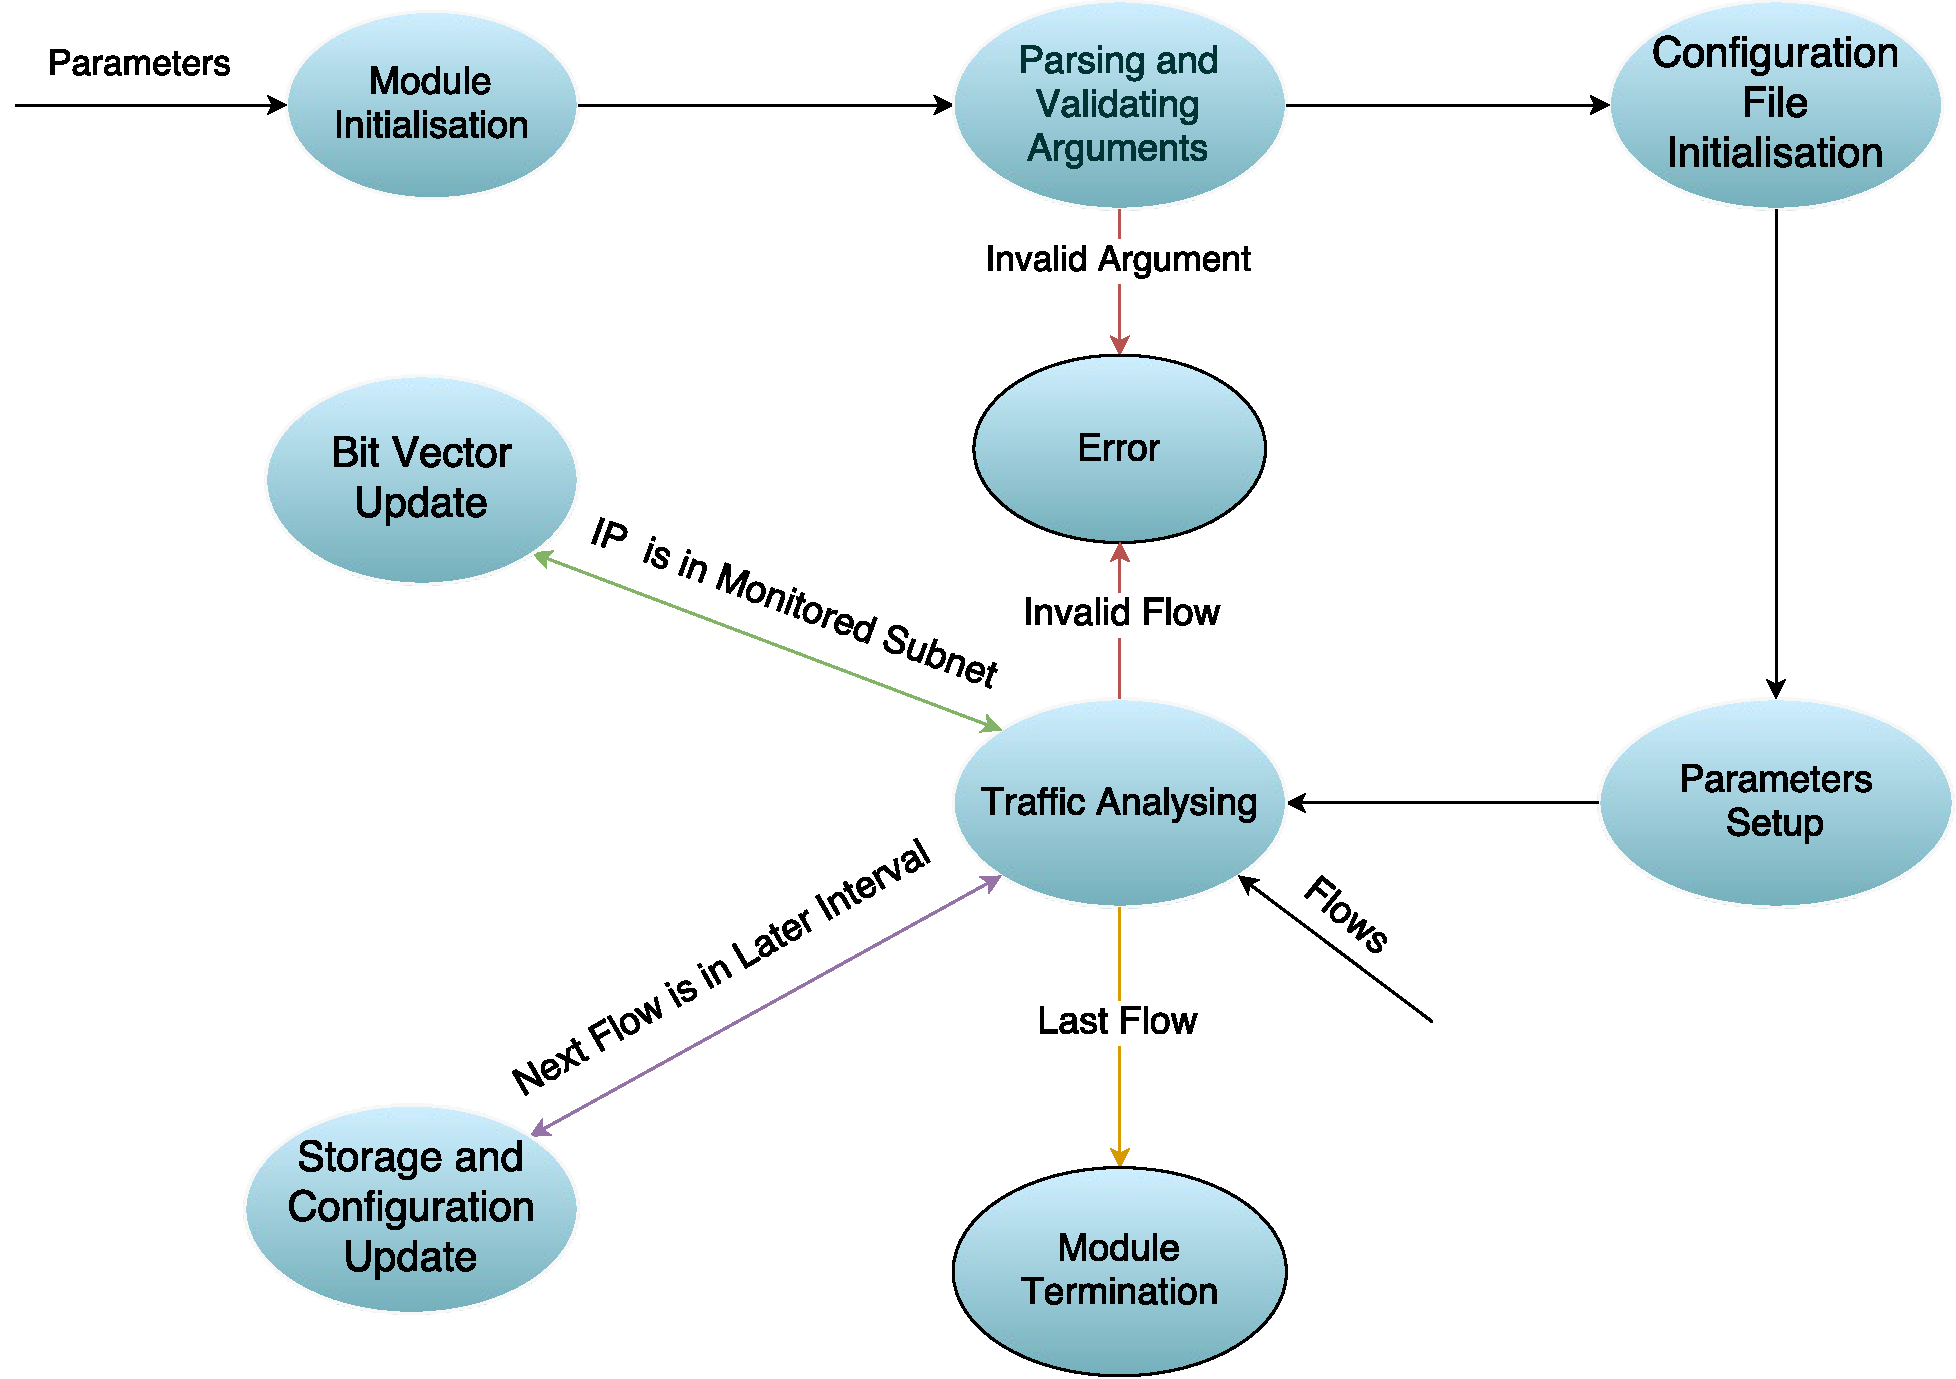
\includegraphics{fig/backend}} \hfill
      \caption{Backend Workflow} \label{fig:backend}
	\end{center}
\end{figure}

The module firstly receives arguments from the user, parses and validates them.

% Parameters
\subsubsection{Parsing and Validating Arguments}\label{sec:backend_params}

Full list of possible parameters (excluding the libtrap common parameters) and their brief description:
\begin{itemize}
  \item \itab{\footnotesize{\texttt{-c/-{}-config\_file}}} \tab{Name of the configuration file. (default: \quotes{config})}
  \item \itab{\footnotesize{\texttt{-d/-{}-directory}}} \tab{Directory for saving bitmaps and configuration. (default: \quotes{.})}
  \item \itab{\footnotesize{\texttt{-f/-{}-filename}}} \tab{Name of bitmap files. (default: \quotes{bitmap})}
  \item \itab{\footnotesize{\texttt{-g/-{}-granularity}}} \tab{Granularity of IPs (subnet size) by a netmask. (default: 8).}
  \item \itab{\footnotesize{\texttt{-r/-{}-range}}} \tab{Range of monitored IPs in format \texttt{<first ip>,<last ip>}.}
  \item \itab{\footnotesize{\texttt{-t/-{}-time\_interval}}} \tab{Time unit for storing data in seconds. (default: 300)}
  \item \itab{\footnotesize{\texttt{-w/-{}-time\_window}}} \tab{Time window of stored data in intervals. (default: 100)}
\end{itemize}

Other parameters that are common for all modules can be found when parameter \texttt{-h trap} is entered.

When the user runs the backend program, they can choose what parameters the original bitmap will have.
The \texttt{-{}-filename} specifies the name of binary storage files and is used as the node name in the configuration file in Section~\ref{sec:config_file}.
The name of the configuration file can be defined by setting \texttt{-{}-config\_file}. If the configuration filename is changed, the changed
name has to be passed to the web server that retrieves the storage statistics from it.

Both the bitmap files and the configuration file are stored to the same directory. By default, it is the current working directory but
it can be changed by the user by setting \texttt{-{}-directory} parameter. If a~custom directory is set, it has to be at the server as well.

The user can also specify the address space, (\texttt{-{}-range}) activity of which will be monitored and its granularity \texttt{-{}-granularity}.
If the address range is not entered, the whole address space of IPv4 is used. In order to create a~reasonable amount of subnets,
granularity default value is set to 8.

Both addresses of the address range must be of the same version and are transformed to the defined granularity during the work flow
(example below in Listing~\ref{lst:range_transf}). Thanks to this transformation,
the subnets can be calculated using the netmask, the size of all subnets
remains the same (whereas if the address space could have customised ending,
the last subnet could end up smaller) and no additional customization has to be done. 

\begin{lstlisting}[label={lst:range_transf},captionpos=b,caption={Address Range Transformation},language=HTML]
   ./ip_activity-r "123.4.5.6,200.0.255.1" -g 16

   Addresses passed to backend:          123.4.5.6 and 200.0.255.1
   Addresses after transformation (/16): 123.4.0.0 and 200.0.0.0
\end{lstlisting}

One time unit for defining subnet activity is specified by \texttt{-{}-time\_interval} in seconds. Time window \texttt{-{}-time\_window}
specifies the maximum intervals stored into the past. After that, the oldest interval is rewritten by the first one as the storage acts like
a~circular buffer.

Example of usage: 
\begin{lstlisting}
   ./ip_activity -i t:12345 -r "1.2.3.4,4.5.6.7" -g 16 -w 250
                 -f "my_bitmap" -t 100 -p
\end{lstlisting}
This sets up the module to store activity about IP addresses \texttt{1.2.3.4} to \texttt{4.5.6.7} by \texttt{/16} subnets,
has a~time interval of 100 seconds and a~time window of 250 intervals. The activity is stored
in files with \textit{my\_bitmap} prefix.

% Configuration file
\subsubsection{Configuration File Initialisation}\label{sec:config_file}
After that, based on the arguments, it opens a~configuration file \texttt{<filename>.yaml}
(if it does not exist, the module creates it first) and adds or rewrites a~node
with the filename of the binary file as the key. By following this pattern, more configurations can be saved in the file.

The backend program does all the needed preparations and fills the statistics, so that the user does not need to add anything on their own
-- and is strongly advised not do that anyway, because changing the values in the configuration file can make the storage unreadable.

The configuration file is used by the backend and the web server for passing the bitmap storage statistics. Therefore,
the filename passed to the backend and the server must be the same (both are set to \quotes{config} by default).
The configuration file is saved to custom directory together with the bitmap files.

The bitmap storage statistics allows the server to access the offsets of
a~particular subnet in the bitmap and visualise binary data in
a~comprehensive manner. This file is in a~YAML~\cite{yaml} format and it
defines ranges of both dimensions and their granularities.
For each distinct configuration, a~new set of binary files is created.

The structure of the configuration file format together with the description of the individual parameters
can be seen in Listing~\ref{lst:config_file}.

\begin{lstlisting}[label={lst:config_file},captionpos=b,caption={Configuration File Structure}]
<filename prefix>:
   addresses:
      granularity: <subnet mask>
      first: <first address>
      last: <last address>
   time:
      first: <timestamp  of the oldest interval in time window>
      last: <timestamp  of the last processed flow>
      granularity: <time unit in seconds>
      window: <number of intervals stored into the past>
      intervals: <number of intervals passed since the beginning>
   module:
      start: <timestamp of the start of the module>
      end: <timestamp of the end of the module>
\end{lstlisting}

All timestamps are in \textit{YYYY-MM-DD HH:MM:SS} format, defined for the local time zone.

An example of such created file is then showed in Listing~\ref{lst:config_file_example}.

\begin{lstlisting}[label={lst:config_file_example},captionpos=b,caption={Configuration File Example}]
mybitmap:
   addresses:
      granularity: 16
      first: 8.0.1.0
      last: 8.3.0.2
   time:
      granularity: 200
      intervals: 150
      window: 100
      first: 2016-04-25 11:04:23
      last: 2016-04-25 13:00:10
   module:
      start: 2016-04-25 11:04:21
      end: 2016-04-25 13:00:15
\end{lstlisting}

While the backend is still running, \texttt{time last}, \texttt{module end} and \texttt{intervals}
values are missing and if the server is started at that point, the frontend considers it an online case.
If all presented values are present, frontend handles it as offline. 

In C++, the work with \texttt{yaml-cpp}~\cite{yaml_cpp} is very intuitive.
The configuration file is loaded into a~node by \texttt{YAML::LoadFile(filename)}.
Accessing nodes is realized by using the keys as indices. For example,
setting the time interval value into the example configuration file
\ref{lst:config_file_example} would look as follows:

\begin{lstlisting}
   YAML::Node config_file = YAML::LoadFile(filename);
   if (config_file == NULL) {
      // Write an error message
      return 1;
   }
   config_file["mybitmap"]["time"]["granularity"] = 200;
\end{lstlisting}

In order to save the changes, modified content of the node has to be streamed into an output stream(\texttt{std::ofstream})
representation of the configuration file.

After setting the configuration, 3\ bitmap files (for source, destination and source + destination addresses)
are created based on the \texttt{-{}-filename} parameter. More information about
the structure of the bitmap files can be found in Section~\ref{sec:bitmap_storage}.

\subsubsection{Parameters Setup}
When analysing the incoming flows, information about IP activity is stored by custom subnets.
That means comparing IPs and calculating the index of the corresponding subnet.

In order to make the process most efficient, all used IPs are logically shifted to the right
so that they only contain bits at indices where the corresponding netmask
has a~value of \quotes{1}.

Calculating the size of the shift:
\begin{lstlisting}[language=C++, captionpos=b, caption={Shift Size Calculation}]
   // IP version derived from entered first and last IP address
   // size of IP version in bits (32 for IPv4, 128 for IPv6)
   int ip_max_prefixlen;

   // ip_granularity is set by user
   // e.g. /12 == 11111111 11110000 00000000 00000000 for IPv4
   int ip_granularity;
   ...
   // 32 - 12 = 20 for IPv4 | 128 - 12 = 116 for IPv6
   int shift = ip_max_prefixlen - ip_granularity;
\end{lstlisting}

Demonstration of shifting:
\begin{lstlisting}
   120.55.246.1/20:
      before shifting:
         binary netmask: 11111111.11111111.11110000.00000000
         binary IP:      01111000.00110111.11110110.00000001
      after 12-bit right shift:
         binary IP:      00000000.00000111.10000011.01111111
         decimal IP:            0.       7.     131.     127
\end{lstlisting}

The shift is performed analogically for IPv6 addresses.

In \texttt{ip\_activity.cpp}, this functionality is implemented by function
\texttt{convert\_to\_granularity (IPaddr\_cpp *addr, int granularity)}.

Before the main loop, the bit vector size is calculated. Normally, the
size would be equal to:

\begin{equation}
   vector\_size = \frac{last\_address - first\_address}{granularity} = \frac{last\_address}{granularity} - \frac{first\_address}{granularity}
\end{equation}

Since both the first and the last address is already shifted, therefore divided by
the granularity, all that needs to be done is the substraction. This operation
is implemented by function \texttt{ip\_substraction (IPaddr\_cpp addr1, IPaddr\_cpp addr2)},
where the result of the function equals $addr2 - addr1$.

In the case of IPv4, the substraction is performed as one operation, using conversion
from IPv4 to \texttt{uint32\_t}, by method \texttt{get\_ipv4\_int()}.
However, when the IP is of version 6, the substraction is divided for the lack
of 128b integer type into 4~parts -- each IPv6
is by \texttt{get\_ipv6\_int()} represented as a~vector of 4~\texttt{uint32\_t}.
The substraction is performed as an N-base substraction (in this case, $2^{32}$ base)
as stated in Listing~\ref{lst:substraction}.

\begin{lstlisting}[label={lst:substraction},captionpos=b, caption={N-base Substraction},language=C++]
// all vectors are of size 4
// ip1 and ip2 have value of corresponding operands 
std::vector<uint32_t> ip1, ip2, result;
uint8_t borrow = 0;

// Go from right to left
for (int i = 3; i >= 0; i--) {
   // If the result is positive, perform normally,
   // clear borrow value
   if (ip2[i] >= (ip1[i] + borrow)) {
      result[i] = ip2[i] - ip1[i] - borrow;
      borrow = 0;
   } else {
      // If the result is negative, add up radix 
      // (here UINT32_MAX) to achieve a positive result
      // and set borrow to 1
      result[i] = ip2[i] + RADIX - ip1[i] - borrow;
      borrow = 1;
   }
}
\end{lstlisting}

The return value of the function is a 32 bits unsigned integer.
If the size of the address space is bigger than \texttt{UINT32\_MAX}, zero
is returned.

\subsubsection{Traffic Analysing}
In the main loop, the module accesses the source and destination address of
each incoming flow. Firstly, the program checks if the current flow belongs
to the most recent interval.

If the flow is older, it is stashed and the program continues with the next one.

If the flow belongs to the later interval, the program assumes that from now on,
all incoming flows have the \texttt{TIME\_FIRST} field greater or equal to this one.
Therefore, it saves the current interval to the storage and if there are
more intervals to be skipped, they are written to the binary file as
intervals with zero activity.

When the interval is set up, the program compares the IP version and
whether the IPs belong to the address range as follows: 

\begin{equation}\label{equ:range}
   first\_ip <= record\_ip <= last\_ip
\end{equation}

When calculating the index to the bit vector, the above mentioned functions
\texttt{convert\_to\_\-granularity (analysed\_ip,\-granularity)} and
\texttt{ip\_substraction(first\_ip, analysed\_\-ip)}
functions are used. The result of the substraction is then in fact a~number of subnets
of chosen granularity between the first address in the range and the analysed IP and
therefore, does not need further calculations and is directly used to access the bit vector.

\subsubsection{Storage and Configuration Update}
Every time a~flow from later interval is encountered, the current bit vector
is passed to function \texttt{binary\_write(filename, bit\_vector, open\_mode, index)}
to be stored to the storage.

If the current number of processed intervals is lower than the time window, data is appended
at the end of the bitmap (therefore, the \texttt{open\_mode} contains \texttt{std::ofstream::app} flag).
Otherwise, based on the passed argument \texttt{index}, the offset of the new beginning of the bitmap
is found (since it is a~circular buffer, it changes after each interval) and the current data
holding information about the oldest interval are overwritten.

Internally, function goes through the vector and aggregates activity data to bytes, so that it can be
stored to the bitmap (more in Section~\ref{sec:bitmap_storage}). and cleared. The principle is
illustrated in pseudocode~\ref{lst:binary_write}.

\begin{lstlisting}[label={lst:binary_write},language=C++]

   // Go through the bit vector
   for (uint64_t i = 0; i < vector.size();) {
      // Initialize each byte to 0
      uint8_t byte = 0;

      // Go through the byte from left to right
      // Set individual bits using a mask byte
      for (uint8_t mask = 128; (mask > 0) && (i < size);
           i++, mask >>=1) {
         if (vector[i]) {
            byte |= mask;
         }
      }

      // Stream bytes to file
      // If size of vector is not divisible by 8,
      // the rest of the byte consists of zeros (padding)
      bitmap.write((const char*)&byte, 1);
   }
\end{lstlisting}

After storing new interval to the storage, the number of the oldest interval in the time window
and the number of passed intervals has changed. To keep the bitmap readable,
these values are updated in the configuration file.

\subsection{IP Address Data Type}
For work with IP addresses, an UniRec class \texttt{ipaddr\_cpp.h}, which has been extended
from its original version in C, is used. Both data types are defined in the Nemea-Framework
repository~\cite{nemeaframework}.
The IP address itself is stored in a~\texttt{ip\_addr\_t union} in big endian.
The union is structurized as follows:

\begin{figure}[H]
   \begin{center}
		\scalebox{0.55}{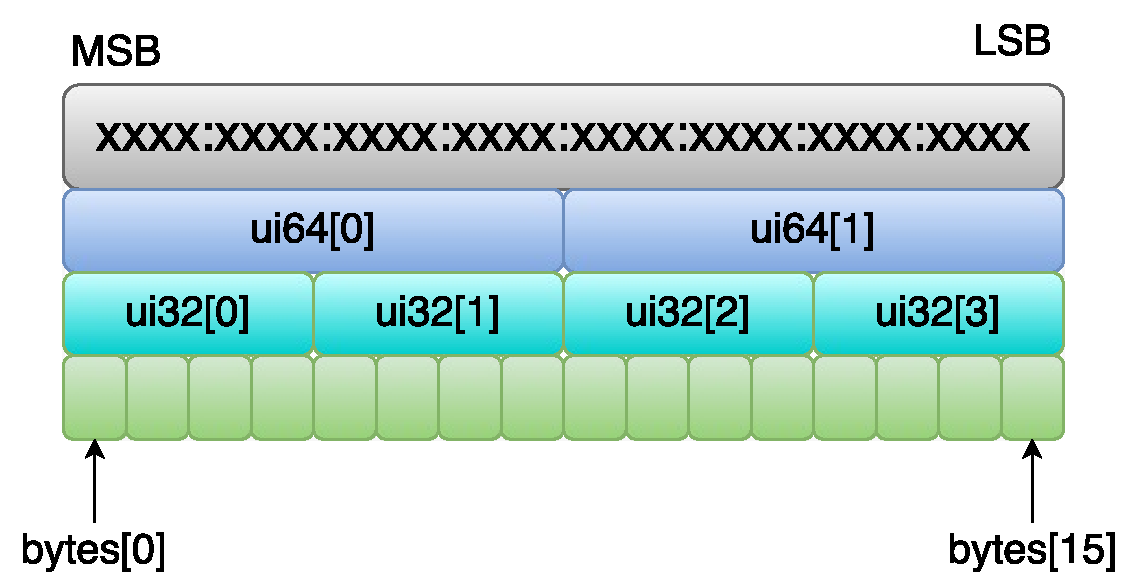
\includegraphics{fig/ip_addr_t}} \hfill
      \caption{\texttt{ip\_addr\_t} union} \label{fig:ip_addr_t}
	\end{center}
\end{figure}

Due to the fact that there are two IP versions, IPv4 and IPv6, each of its own size,
their location in the \texttt{ip\_addr\_t} is different. Wherease IPv6 simply occupies
all 16 bytes, IPv4 is starts at the 9th byte. Internally, the union for IPv4 looks as follows:

\begin{figure}[H]
\begin{center}
   \begin{lstlisting}
      0000:0000:0000:0000:<ipv4 address>:ffff:ffff
   \end{lstlisting}
\end{center}
\end{figure}


% Bitmap Storage
\section{Bitmap Storage}\label{sec:bitmap_storage}
The main storage is a set of 3~files in a~binary format, one for each type of address
(source addresses, destination addresses, either of the two). It is used for storing big
amounts of data efficiently, using one bit for defining state of a given subnet
at a~given moment. As the result, structure has two dimensions, One row represents an
activity of the whole monitored address space in one time interval.

The storage works as a~circular buffer. When the storage reaches the time window limit,
the oldest data is rewritten. Therefore, when the online mode is chosen, the frontend
has to calculate the beginning from the time of the first record as follows:

\begin{equation}\label{equ:range}
   intervals = time\_first + intervals\_passed \times time\_unit
\end{equation}

The bitmap \texttt{filename} uniquely identifies a~set of bitmaps and their configuration.
The name of each bitmap file is created by appending \quotes{\texttt{\_<type>.bmap}} to \texttt{filename}.
Possible types are defined as follows -- \texttt{s} (source address), \texttt{d} (destination address)
and \texttt{sd} (source or destination address). It is stored in the same directory as the
configuration file.

When storing data, it is more efficient to see a~row as one unit of time. It is much easier to concatenate/rewrite one line in
a~binary file than to go through the file and add one symbol at the end of each line. Therefore, in the NEMEA module where
the speed of data processing is essential, the matrix is structured this way.

Since the size of the bit vector does not need to be divisible by 8, there is a~padding
at the end of each line to the nearest byte. The padding is the only part of the storage
that is not used for storing the activity.

The index for accessing wanted time interval is calculated as follows:

\begin{equation}
offset = interval\_position\_in\_time\_window \times CEILING(\frac{vector\_size}{8})
\end{equation}

When accessing data from the web server, the resulting image uses $x$-axis (columns) for displaying time units,
whereas in the storage, it is represented by rows. Therefore, after each query,
the server transposes the bitmap before any other specified operation needed for data visualisation.

As for the size of the bitmap file, both maximum size of the bit vector and the time window
size are set to 1000 for the option of displaying the bitmap 1:1 conveniently. The limits
are set in macros \texttt{MAX\_WINDOW} and \texttt{MAX\_VECTOR\_SIZE} and can be changed.

Following equations demonstrate the efficiency of the storage and the size of part occupied by padding bits.

Conditions that must be met for all equations:
\begin{align*}
   &intervals \in \langle 0; time\_window \rangle \\
   &time\_window \le MAX\_VECTOR\_SIZE \\
   &vector\_size \le MAX\_VECTOR\_SIZE
\end{align*}

Size of the bitmap storage file can be calculated as follows:
\begin{align*}\label{equ:bitmap_size}
   &bitmap\_size = size\_of\_interval \times intervals\:[B] \\
   &bitmap\_size = CEILING(\frac{vector\_size}{8}) \times intervals\:[B]
\end{align*}

Size of the padding in bitmap storage is expressed as follows:
\begin{align*}
   &padding\_size = size\_of\_padding\_in\_vector \times intervals\:[b] \\
   &padding\_size = ((8 - (vector\_size\mod 8))\mod 8) \times intervals\:[b]
\end{align*}

Based on the size of the padding and the storage itself, let us express what percentage
of the storage is occupied by padding:
\begin{align*}
   &padding\_part = \frac{padding\_size}{bitmap\_size} \times 100\% \\
   &padding\_part = \frac{((8 - (vector\_size\mod 8))\mod 8) \times intervals}{CEILING(\frac{vector\_size}{8}) \times intervals \times 8} \times 100\% \\
   &padding\_part = \frac{((8 - (vector\_size\mod 8))\mod 8)}{CEILING(\frac{vector\_size}{8}) \times 8} \times 100\%
\end{align*}

As the equation is reduced, it is clear that the part occupied by padding is influenced by vector size and its divisibility by 8. The graph~\ref{fig:padding}
shows the relationship between the vector size on $x$-axis and percentage of padding in storage on $y$-axis. The part
containing padding bits is getting relatively smaller to the bitmap storage with increasing vector size.

\begin{figure}[H]
\begin{center}
      \scalebox{0.45}{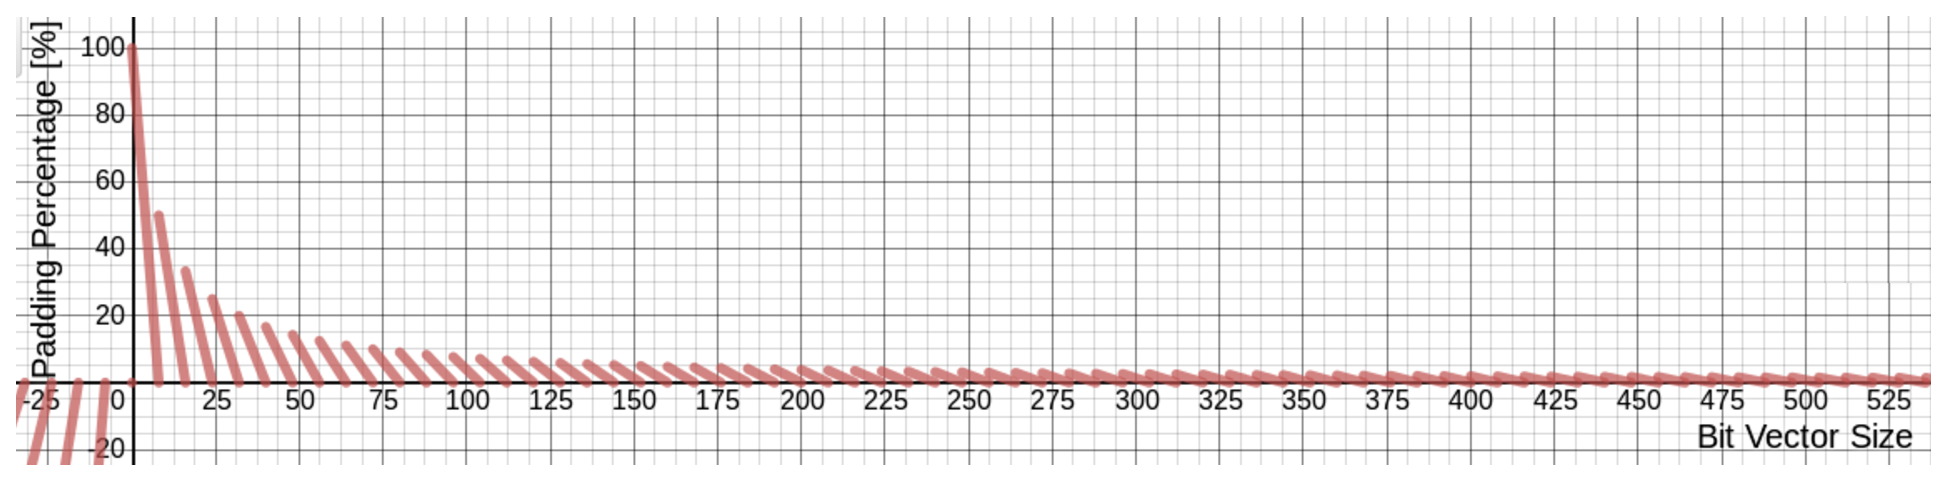
\includegraphics{fig/padding}} \hfill
      \caption{Padding percentage based on vector size} \label{fig:padding}
\end{center}
\end{figure}

Let us take the maximum size of bitmap and maximum padding for illustration,
how much of the storage space the padding can occupy at most at default limits.
The size of the vector equals 993 for it is the biggest value below
\texttt{MAX\_VECTOR\_SIZE} that has the most (7) padding bits.

\begin{align*}
   &intervals = 1000 \\
   &vector\_size = 993 \\
   \\
   &padding\_part = \frac{((8 - (vector\_size\mod 8))\mod 8)}{CEILING(\frac{vector\_size}{8}) \times 8} \times 100\% \\
   &padding\_part = \frac{((8 - (993 \mod 8))\mod 8)}{CEILING(\frac{993}{8}) \times 8} \times 100\% \\
   &padding\_part = \frac{((8 - 1)\mod 8)}{125 \times 8} \times 100\% \\
   &padding\_part = \frac{7}{1000} \times 100\% = 0.7\%
\end{align*}

For 1000 intervals and vector size 993, the percentage is mere $0.7\%$. The rest $99.3\%$ of the size is occupied by needed data.

When compared to querying data in whole flow records where only one attribute of the whole record is used,
the ratio of the stored data to used data here is significantly better.




% Web server
\section{Web Server}
The web server is implemented in the source file \textit{http\_server.py}. For bitmap handling,
the server uses the visualisation handler (discussed in Section~\ref{sec:visualisation_handler}).

The server is compatible with both Python 2.x and Python 3.x versions.
In order to run the server, several non-standard packages have to be installed for chosen
version of Python (see subsection~\ref{sec:python_packages}).

The server program creates a~new class of a~HTTP request handler and passes it the input
arguments and the visualisation handler. Then, the program creates a~socket, binds it
to the defined port and enters an endless loop.

In order to visualise valid data, the server program cannot be initiated
until the backend program is activated and the configuration is written in the
dedicated file. Also, if backend is run again with a different configuration
but the same file names, the server has to be restarted.

\subsection{Workflow}
The main functionality of the server is present in Figure~\ref{fig:server}.
The scheme is simplified in order to demonstrate the main operations more clearly.

\begin{figure}[H]
   \begin{center}
		\scalebox{0.4}{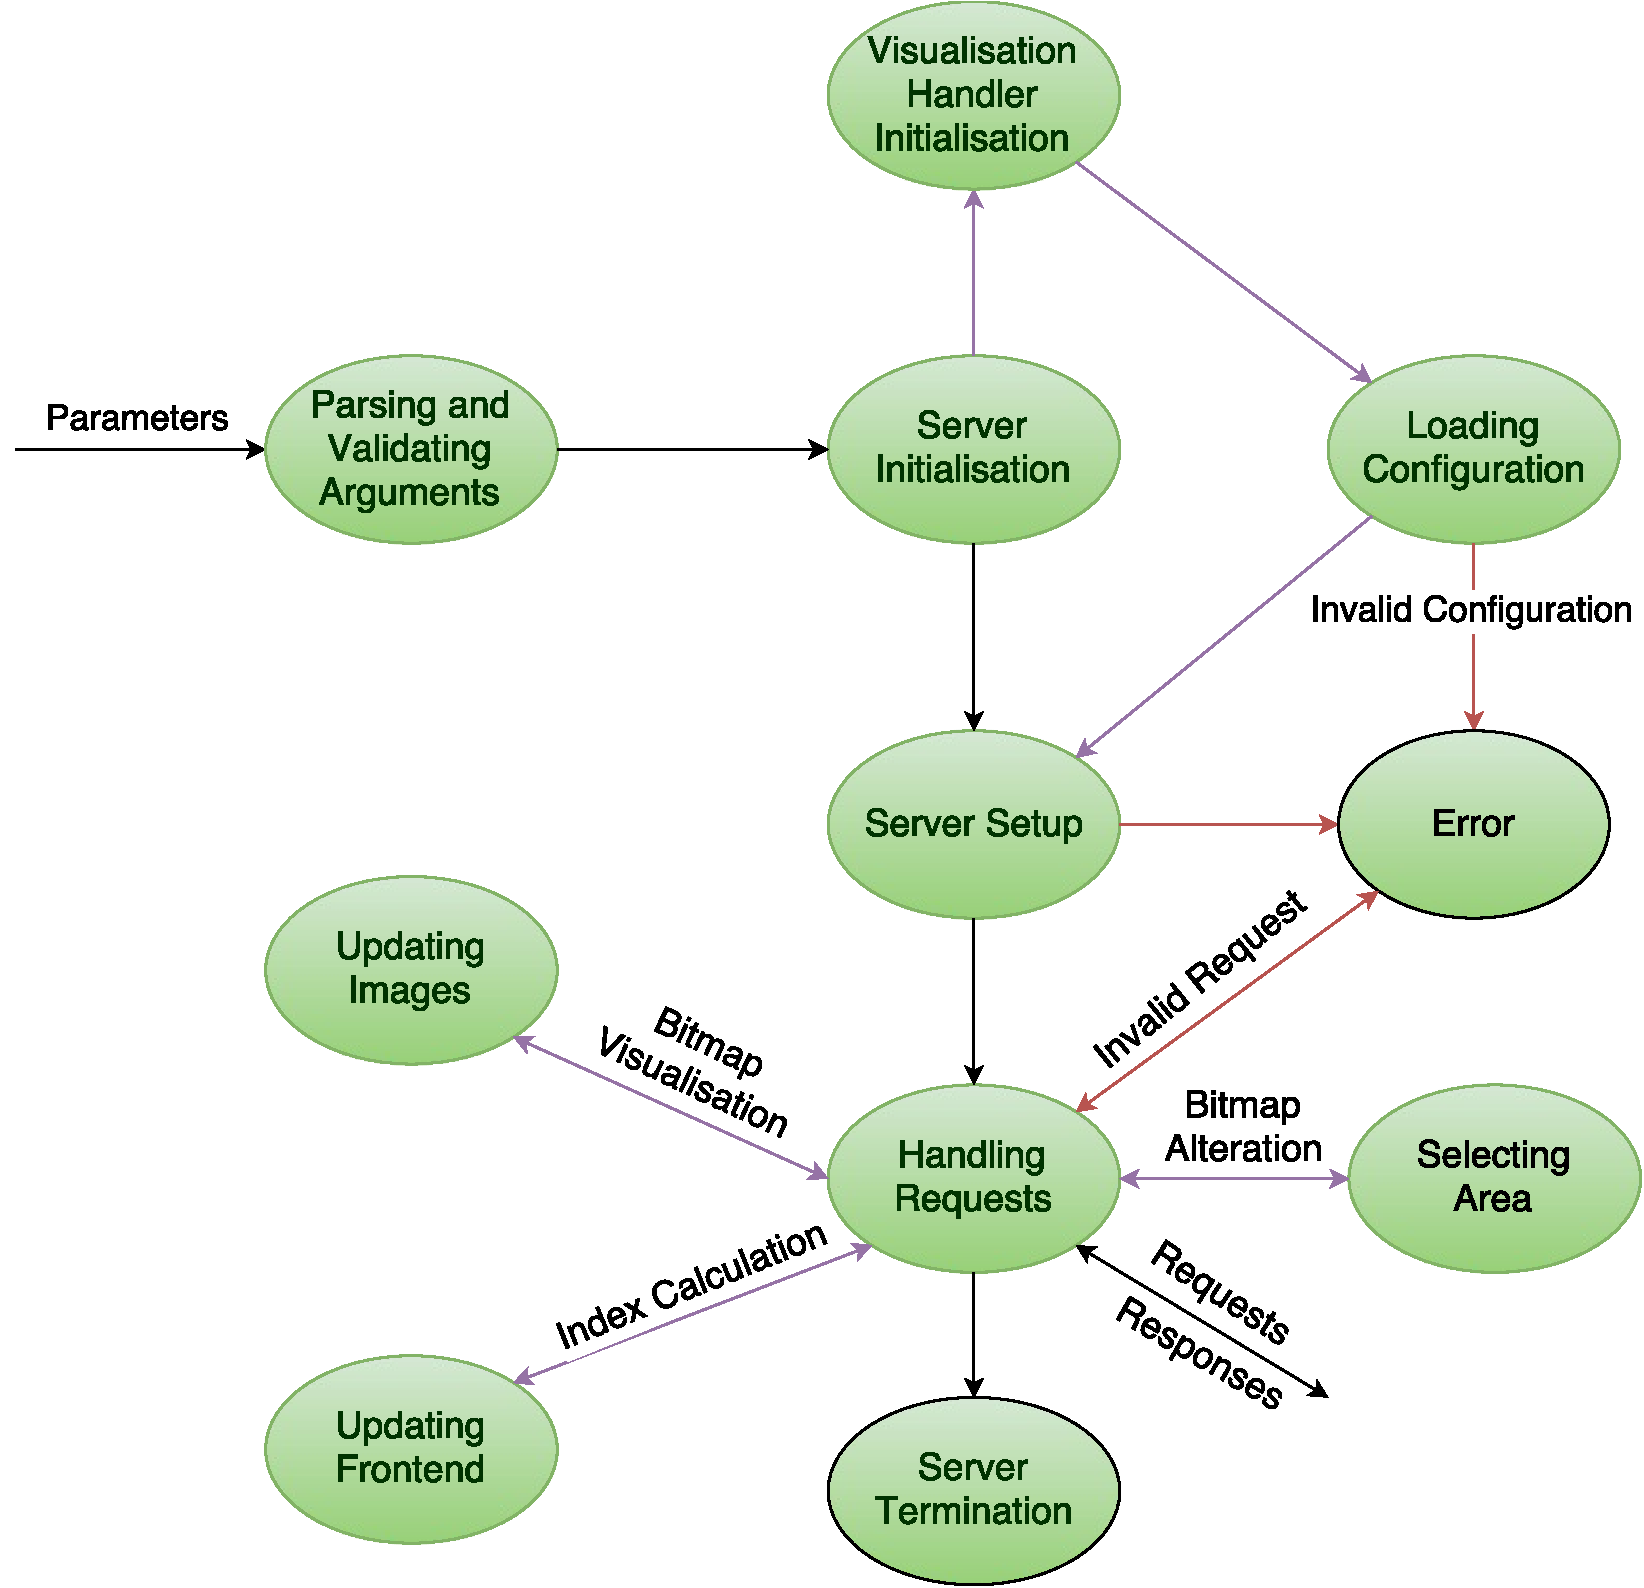
\includegraphics{fig/server}} \hfill
      \caption{Web Server Workflow} \label{fig:server}
	\end{center}
\end{figure}

The start state is initiated by running the program with custom parameters.
The end states are similarly to the backend scheme defined by a~black
perimeter line. The server can be terminated unsuccessfully before entering
serving loop when an error occurs or successfully when an interruption (\texttt{SIGINT})
or terminating (\texttt{SIGTERM}) signal is received. If an error occurs while
the server is active, the error message is sent to the standard error output
but the server keeps running.

Since the server uses the visualisation handler module, its actions are also added
to the scheme, distinguished by purple arrows. Its initialisation takes place
right before server setup when the handler object is added to the request handler
class as an attribute. Other interactions with the visualisation handler are
visible during the request processing where it is the main source of
data and enables the server to manipulate it.

One of the states is not addressed directly but discussed in several section.
This state is called \textit{Updating Frontend} and it includes sending the
main page to the client and calculating the index values of current cursor position.

\subsubsection{Parsing and Validating Arguments}\label{sec:server_params}
At first, the program parses arguments by the user using the \texttt{argparse}~\cite{argparse} package.
The list of the possible parameters is as follows:

\begin{itemize}
  \item \itab{\footnotesize{\texttt{-c/-{}-config\_file}}} \tab{Filename of the configuration file. (default: \quotes{config})}
  \item \itab{\footnotesize{\texttt{-d/-{}-dir}}} \tab{Path to directory with configuration and bitmaps (default: \quotes{.})}
  \item \itab{\footnotesize{\texttt{-f/-{}-filename}}} \tab{Filename of bitmap storage files. (default: \quotes{bitmap})}
  \item \itab{\footnotesize{\texttt{-H/-{}-hostname}}} \tab{Hostname of the server. (default: \quotes{localhost})}
  \item \itab{\footnotesize{\texttt{-p/-{}-port}}} \tab{Server port. (default: 8080)}
\end{itemize}

The user can specify the configuration filename by passing \texttt{-{}-config\_file}. This approach is needed if the user
decided to change the configuration filename in backend. To find the used configuration, the user has to define
the filename of the bitmaps using \texttt{-{}-filename} parameter that will serve as key in the configuration file to the bitmap parameters.

The server can be run from other directory than the configuration and bitmap files are located in.
In that case, the path to the custom directory has to be specified by \texttt{-{}-dir} parameter.

If the user wishes to identify the server with custom hostname or port,
they can define the \texttt{-{}-hostname} or \texttt{-{}-port} parameter,
bearing in mind the well-known ports~\cite{port_registry} (range 0-1023)
where they need a~root permission.

The received arguments are parsed and validated by the program and then the bitmap parameters are retrieved.

\subsubsection{Server setup}
The server retrieves bitmap statistics from the configuration file
(more about its structure in Section~\ref{sec:config_file}) based
on its filename using the \texttt{Visualisation\_Handler} object.
This process is described in Section~\ref{sec:loading_config} where the additional
module is described in more detail.
After the parameters initialisation, the creation od the request handler is initiated.

In order to be able to handle various requests from the client, the basic request handler class is modified.
In function \texttt{create\_handler(arguments, visualisation\_handler)}, the program sets parameters of the bitmap storage based on the
configuration file and defines a~new class \texttt{My\_RequestHandler} that is inherited from the \texttt{BaseHTTPRequestHandler} class
and extends its functionality for its intended use -- retrieving and editing bitmap and converting bitmap to image.

Subsequently, the \texttt{My\_RequestHandler} class together with the defined socket pair \texttt{<hostname> :<port>}~are used for creating
the HTTP server.

\subsubsection{Handling Requests}
The program then enters an infinite loop where the server listens for incoming requests. All errors occurred
during this state can produce an error message but they do not end the loop.
The activity of the server can only be stopped by incoming interruption (\texttt{SIGINT})
and termination (\texttt{SIGTERM}) signals.

Since the processed requests are tied up to both the server and the web client, they are discussed
separately in Section~\ref{sec:requests}.



% Visualisation Handler
\section{Visualisation Handler}\label{sec:visualisation_handler}
The bitmap manipulation used by the server is defined in a~separate file called
\textit{activity\_visualisation.py}. It stores all the bitmap configuration and
also the current bitmap for visualisation.

\subsection{Loading Configuration}\label{sec:loading_config}
In order to fill the handler with correct values, its method \texttt{load\_config(dir, bitmap\_name, config\_\-name)} is
called. In this method, the handler stores all the bitmaps and their parameters retrieved from the configuration
file using \textit{pyyaml} package. This package uses the same approach as is done in backend --
the values are accessed using keys as indexes to the file structure. Beside the configuration file values,
similarly to the backend, the handler calculates the size of the address space to be able to index data in the storage.

Then, the handler is called solely for manipulating the bitmap and its statistics.
It always stores bitmap internally in ratio 1:1 and scales the image only for the client based on
their request.

\subsection{Functionality}\label{sec:handler_functionality}
As stated above, the main functionality of the visualisation handler is manipulating
the binary storage and retrieving its data. In this part of the thesis,
the main operations are introduced.

\subsubsection{Index Calculation}\label{sec:indexing_principles}
One type of operation implemented is getting a~data offset from data value and vice versa. This is used
for example when calculating the current position of the client's cursor.

The principle of the former operation (offset from value) can be defined as follows:
\begin{equation}
   offset = \frac{current\_value - min\_value}{granularity}
\end{equation}

The latter operation (value from offset) can require additional adjustment due to used units, for
example transforming offset to seconds to calculate time. The process can be described followingly:
\begin{equation}
   value = min\_value + offset\_in\_units
\end{equation}

\subsubsection{Retrieving Bitmap}
Other functionality is retrieving bitmap from the storage (implemented in
\texttt{binary\_read( bitmap\_name)}).
The principle is demonstrated in Figure~\ref{fig:bitmap_retrieval} with the size
of address space equal to 10, time window 100\ intervals and current offset 1~(of the newest interval).

\begin{figure}[H]
   \begin{center}
		\scalebox{0.45}{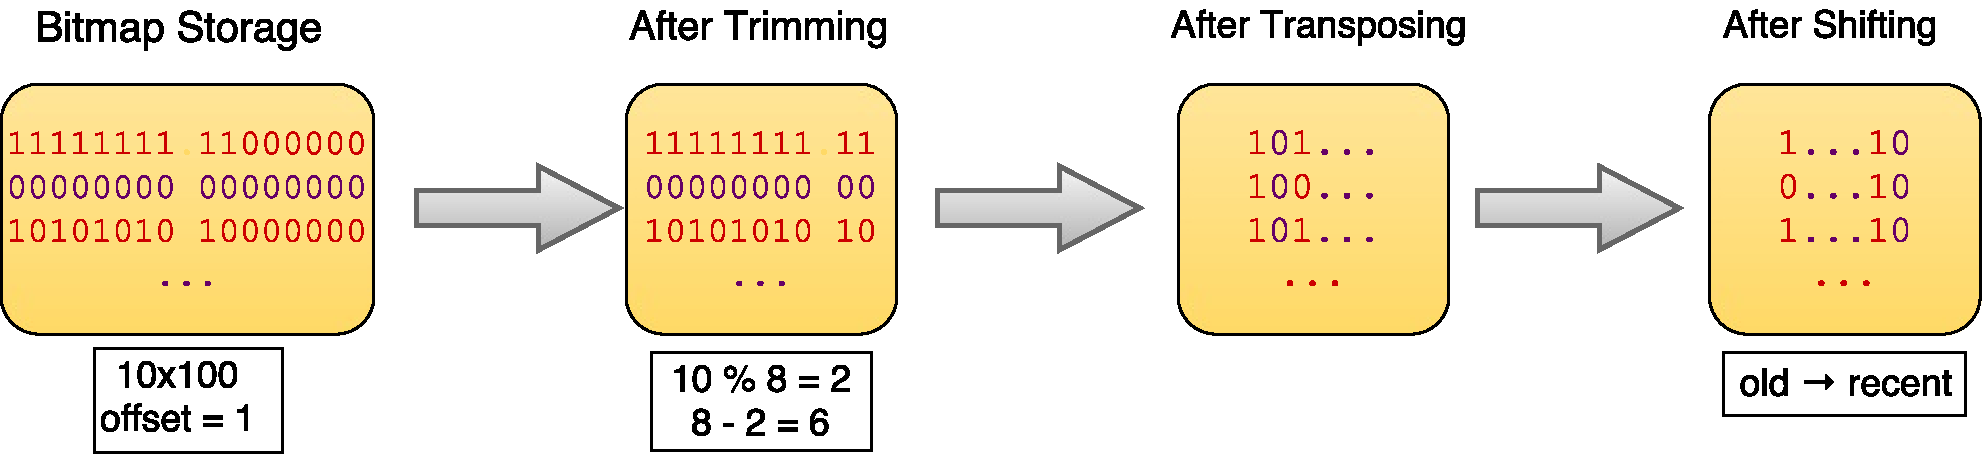
\includegraphics{fig/bitmap_retrieval}} \hfill
      \caption{Bitmap Retrieval} \label{fig:bitmap_retrieval}
	\end{center}
\end{figure}

The handler reads the content of the binary file and trims the padding bits from each row.
It then transposes the 2D array so that each row contains information about one subnet.
Finally, the handler shifts each row based on the offset of the beginning of
the circular buffer to increase readability of the final image.

\subsubsection{Creating or Updating Images}
Retrieving bitmap data is usually followed by creating the image based on the bitmap
(\texttt{create\_image(bitmap, filename, scaleR, scaleC, height, width, selected)}).
The final image always has the same proportions $subnet\_size:time\_window$. If the
whole image is not filled with storage data, the rest is set to an \textit{undefined}
value distinguished by gray colour. The original data always covers the top left corner.

In the case of original bitmap, the handler takes the bitmap and scales it in passed ratio
 -- rows by \texttt{scaleR}:1, columns by \texttt{scaleC}:1. If the bitmap does not
 cover the whole time window, the rest of the image is going to have \textit{undefined} value.
 
When creating selected area image, the selected data scaling units are calculated in advance,
so that the image is as big as possible without exceeding the size of the original one.
When creating the image, only the remaining part of the image, here without scaling, is
set to \textit{undefined}.

Passed bitmap is loaded to a~1D buffer. Each bit is then transformed into one pixel --
\quotes{0} $\rightarrow$ RGB(0,0,0), \quotes{1} $\rightarrow$ RGB(255,255,255) and
\textit{undefined} $\rightarrow$ RGB(105,105,105). The shade can be customized
by changing \texttt{undefined} attribute. Created image is then saved
to an image file specified by \texttt{filename}.

\subsubsection{Area Selection}
When client wants to select an area of the bitmap, they select the edges of this area --
$x_{min}, x_{max}, y_{min}, y_{max}$ and submit the request to the server. The job of
the visualisation handler is to crop the original bitmap and leave only the selected area
which is implemented in \texttt{edit\_bitmap(query)} method, leaving only the
defined ranges:

\begin{lstlisting}[language=Python]
   selected_bitmap = original_bitmap[x_min:x_max][y_min:y_max]
\end{lstlisting}

The selected bitmap is then scaled in a~maximum possible way that
does not exceed the size of the original bitmap. The principle is
formally defined in Figure \ref{fig:selected_scaling}.
\begin{figure}[H]\label{fig:selected_scaling}
   \begin{align*}
      &\mbox{let } x_{selected} = x_{max} - x_{min}; y_{selected} = y_{max} - y_{min}; X,Y \subset \mathbb{N}\\
      &\forall x \in X \mbox{ that } x \cdot x_{selected} \le address\_space \rightarrow x \in X_{2}\\
      &\forall y \in Y \mbox{ that } y \cdot y_{selected} \le time\_window \rightarrow y \in Y_{2}\\
      &x_{scale} = max(X_2), y_{scale} = max(Y_2)
   \end{align*}
\end{figure}
Thanks to this scaling, the client can inspect is area of interest more closely -- be it IP subnets or
specific intervals. The result is sent to the client.




% HTTP Requests
\section{HTTP Requests and the Corresponding Responses}\label{sec:requests}
The server has modified HTTP GET request handler, so that the web client can request various specific data.
The other request methods~\cite{request_methods} are handled by default handlers in the \texttt{BaseHTTPRequestHandler} class.
The GET method is handled by class method \texttt{do\_GET()}. Based on the requested resource (identified
by URI~\cite{uri}), the server generates the response.

The server has implemented behaviour for several types of requests.
In this section, the formats of valid requests are shown and the principle of server's handling is demonstrated.

% Main page
\subsection{Main Page}
The most basic one is requesting the main page which can be identified as \quotes{\textit{/}},
\quotes{\textit{/index.html}} or \quotes{\textit{/frontend.html}} as it is physically stored in \texttt{frontend.html}.
In order to send valuable information back to the client containg the statistics of the bitmap file, the server modifies
the contents of the \texttt{frontend.html} file, adding current storage information to the \textit{Characteristics} section.
Using the package \textit{BeautifulSoup}, the file is parsed and the information is formatted and appended to the designated elements.

% Image update
\subsection{Updating Image}
Another type of request is used for updating the image. When the online mode is
active, the client sends the asynchronous update request periodically. The update interval can be changed in the frontend file
\textit{frontend.js} by setting \texttt{update\_interval} value and is set to 30 seconds by default. In the case
of offline mode, client sends update request only when the page is refreshed. In both modes, the server loads the
new storage contents (provided they exist), visualises the data in defined scaling and sends an encoded image back to the client.

The URI of the request for updating the image looks as follows:

\begin{lstlisting}[language=HTML,label={lst:update_req}]
   GET /<path to image>?update=true&scale=<ratio> HTTP/<version>
\end{lstlisting}

The request consists of the path to the image that is consistent -- \quotes{images/image\_<bitmap type>.png},
so that the bitmap type does not need to be specified separately.
To indicate this type of the request, the type \texttt{update} with symbolic value is added to the URI.
Since the user can also set scaling of the image, it also specified in the URI format.

The response to this request depends on if the requested bitmap exists. If it does not,
the server responds with a~response header of the following format:

\begin{lstlisting}[language=HTML,label={lst:update_resp_none}]
   HTTP/<version> 404 Not Found
   Bitmap: none
\end{lstlisting}

If the bitmap does exist, after creating the image of specified characteristics,
the following reponse is sent back:

\begin{lstlisting}[language=HTML,label={lst:update_resp_ok}]
   HTTP/<version> 200 OK
   Content-Type: image/png
   Interval_range: <range>
   Mode: <online/offline>
   Bitmap: ok

   <base64 encoded image>
\end{lstlisting}

In this response, the number of displayed interval range is sent together with
the current mode, so that the client can react to the change from online
mode to offline. \texttt{Bitmap: ok} indicates that the client can decode
the received response and display the result to the user. 

% Selecting Area
\subsection{Area Selection}
The next request is sent when only a~specific area of the image is to be
displayed in a~dedicated element.
The server creates a~new image from the original bitmap based on the query
values, scales it (principle demonstrated in formal definition in Figure~\ref{fig:selected_scaling})
and sends it back to the client in the response.

The request has the following format:

\begin{lstlisting}[language=HTML,label={lst:select_area}]
   GET /?select_area=true&bitmap_type=<type>&
       first_ip=<ip>&last_ip=<ip>&
       first_time=<time>&last_time=<time> HTTP/<version>
\end{lstlisting}

The parameters consist of the limits of the specified area and the
bitmap type.

If the original bitmap does not exist, the server sends only a header
informing that no bitmap is available:

\begin{lstlisting}[language=HTML,label={lst:select_area_resp_none}]
   HTTP/<version> 404 Not Found
   Bitmap: none
\end{lstlisting}

If the bitmap does exist, the server sends the encoded image visualising the specified area
together with the scaling ratios of both dimensions as demonstrated here:

\begin{lstlisting}[language=HTML,label={lst:select_area_resp_ok}]
   HTTP/<version> 200 OK
   Content-Type: image/png
   IP_unit: <scaling of IP subnets>
   Time_unit: <scaling of time intervals>
   Bitmap: ok

   <base64 encoded image>
\end{lstlisting}

%Index Calculation
\subsection{Index Calculation}
This request type is used for finding the IP subnet and time interval value at a~given index.
When the user hovers over the image, the IP subnet and the interval is displayed in the dedicated table \textbf{Current Position}.
Since JavaScript does not have any convenient library that would add up an IP address (possibly an IPv6 in the reduced form)
and an integer, it is easier to get the value from the server that is able to implement this functionality using
\textit{ipaddress} package. And while doing that, it also calculates the interval index.

The position is calculated for currently displayed image, so that the frontend
only needs to specify whether the operation is to be
carried out on the original bitmap or the selected area.
Related calculation methods are discussed in Section~\ref{sec:handler_functionality}.

The request format looks as follows:

\begin{lstlisting}[language=HTML,label={lst:current_position}]
   GET /?calculate_index=true&bitmap_type=<type>&
       first_ip=<ip>&ip_index=<index>&
       first_time=<time>&time_index=<index> HTTP/<version>
\end{lstlisting}

This format is distinguished by the type \texttt{calculate\_index}. It contains
the bitmap type that specifies if the current position is to be calculated for
the original bitmap or the selected area. Besides that, the first values in
both ranges altogether with current indices are inserted and passed to the
server methods responsible for the calculation. 

After computing the values, the server sends the following response to the client:

\begin{lstlisting}[language=HTML,label={lst:current_position_resp}]
   HTTP/<version> 200 OK
   Content-Type: text/plain
   IP_index:<calculated IP at index>
   Cell_colour:<colour of the current position>
   Time_index:<calculated time at index>
\end{lstlisting}

The response is in the plain text format and it consists of both
IP and time values at the specified indices. The values are sent in
headers \texttt{IP\_index} and \texttt{Time\_index}. If the user hovers
over an area with undefined values, both values equal \texttt{\quotes{undefined}}.

In order to illustrate the current position activity
status, the colour representing the activity at specified coordinates is sent
as a~string (\quotes{\textit{white}} for active, \quotes{\textit{black}} for inactive or
\quotes{\textit{gray}} for undefined). 



%Client
\section{Web Client}
The web client is implemented in source files with the \textit{frontend} filename. It
consists of a~HTML file with the basic page content, CSS stylesheet and JavaScript
file describing the page behaviour. The webpage layout is discussed further in Section
\ref{sec:client_design}.

The client displays the monitored activity to the user. All the data is supplied
to the frontend by the server in the form of a~HTTP response.

\subsection{Page Content}
The main page content is defined in \textit{frontend.html} and used stylesheet
in \textit{frontend.css}. Since the
displayed information changes based on monitred traffic, some of the elements
are added or modified dynamically by JavaScript.

\subsubsection{Original Bitmap}
The top part of the main page is displayed in Figure~\ref{fig:main_page} and
is dedicated to the visualisation of the whole bitmap.
It is divided into several areas. The left column is dedicated to data
statistics and the right one is used for modifying the image.

\begin{figure}[H]
   \begin{center}
		\scalebox{0.5}{\frame{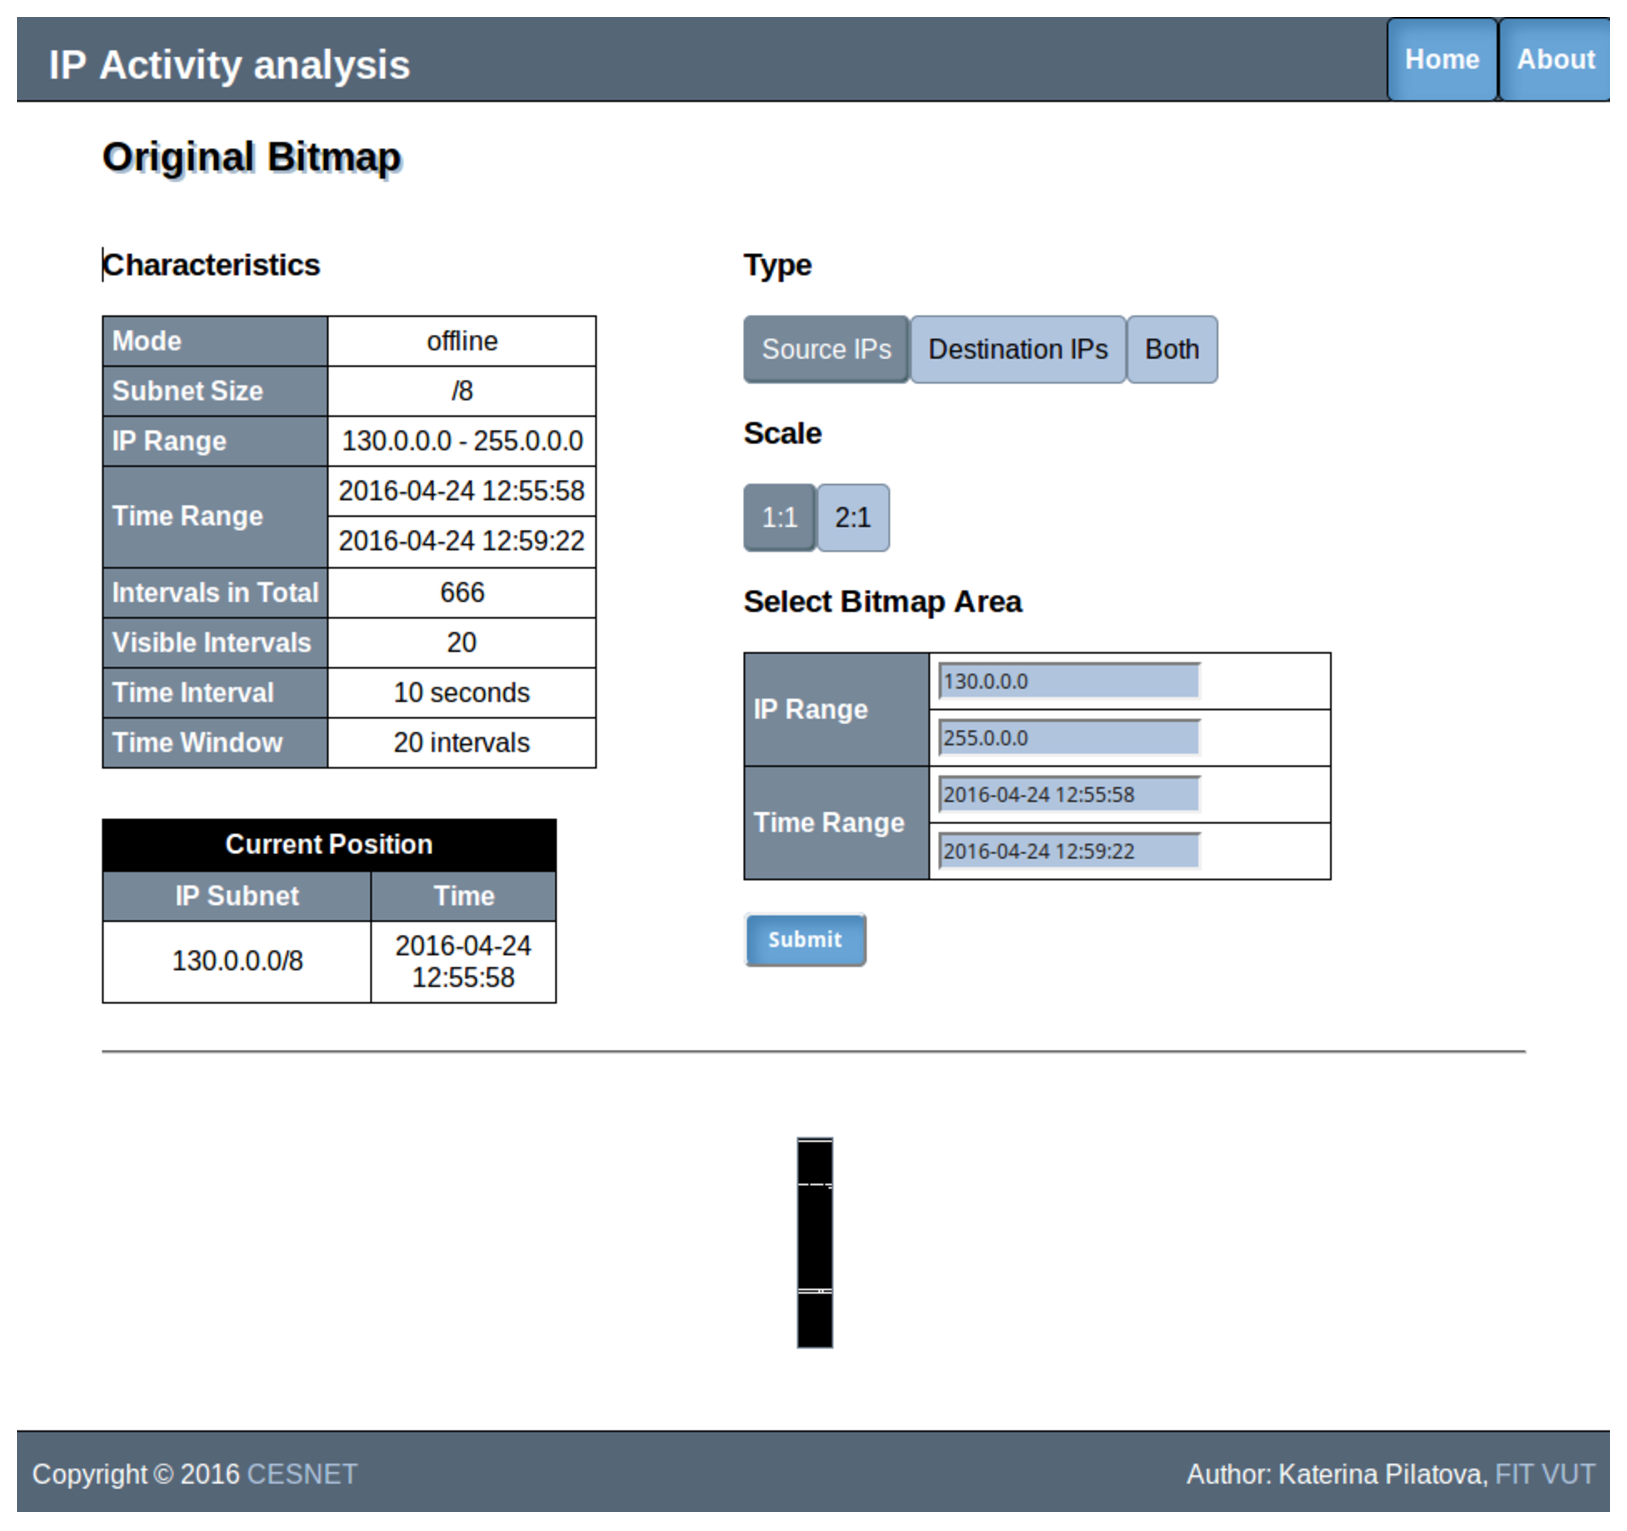
\includegraphics{fig/main_page_1}}} \hfill
      \caption{Frontend Main Page} \label{fig:main_page}
	\end{center}
\end{figure}

The \textbf{Characteristics} area contains bitmap statistics and its purpose
is to improve the readability of the visualised activity. The user has
better idea about the units in both dimensions and knows which data are
currently displayed.

The full list of the characteristics and their brief description can be found below:

\begin{itemize}
   \item \itab{\footnotesize{Mode}} \tab{Mode the activity monitoring is in. Value: \textit{online} or \textit{offline}.}
   \item \itab{\footnotesize{Subnet Size}} \tab{Size of the network mask dividing monitored address space.}
   \item \itab{\footnotesize{IP Range}} \tab{Contains monitored IP range. Value: \textit{<first IP> - <last IP>}}
   \item \itab{\footnotesize{Time Range}} \tab{Contains visible interval range as timestamps.}
   \item \itab{\footnotesize{Intervals in Total}} \tab{Total number of scanned intervals by backend module.}
   \item \itab{\footnotesize{Visible Intervals}} \tab{Number of currently visible intervals. Value: $0-time\_window$}
   \item \itab{\footnotesize{Time Interval}} \tab{Size of one time interval in seconds.}
   \item \itab{\footnotesize{Time Window}} \tab{Size of the time window in intervals.}
\end{itemize}

Below the characteristics is located the \textbf{Current Position} which
changes dynamically as the user's cursor moves over the image area. The
background reflects the activity status of the current coordinates and
the exact values of the subnet and time interval coordinates are also included.
If user hovers over the area with undefined values, corresponding values are set to
\textit{undefined}.

The user can change the displayed bitmap type (section \textbf{Type}) and
scale image so that the smaller areas are more visible (section \textbf{Scale}).
The user can also select area they would like to examine in detail by
changing the IP or time range values in the form and submitting the form.
After submitting the form, a~previously hidden area with information
about the specified ranges is now visible.

Under the statistics and options, the visualised activity is displayed as an image.
Black areas indicate inactivity, white areas active subnets and gray areas undefined
values. The interface enables the user to interact with the image.

The user can hover over the image to display activity of a~certain position
or select area by clicking on a~chosen position and dragging pointer to the chosen
range limit, creating a~frame around chosen area in the process (see Figure~\ref{fig:drag1}.
The user can drag the pointer in any direction. If the user does not drag
in left-to-right top-to-bottom direction, the values are automatically swapped.

\begin{figure}[H]
   \begin{center}
		\scalebox{0.68}{\frame{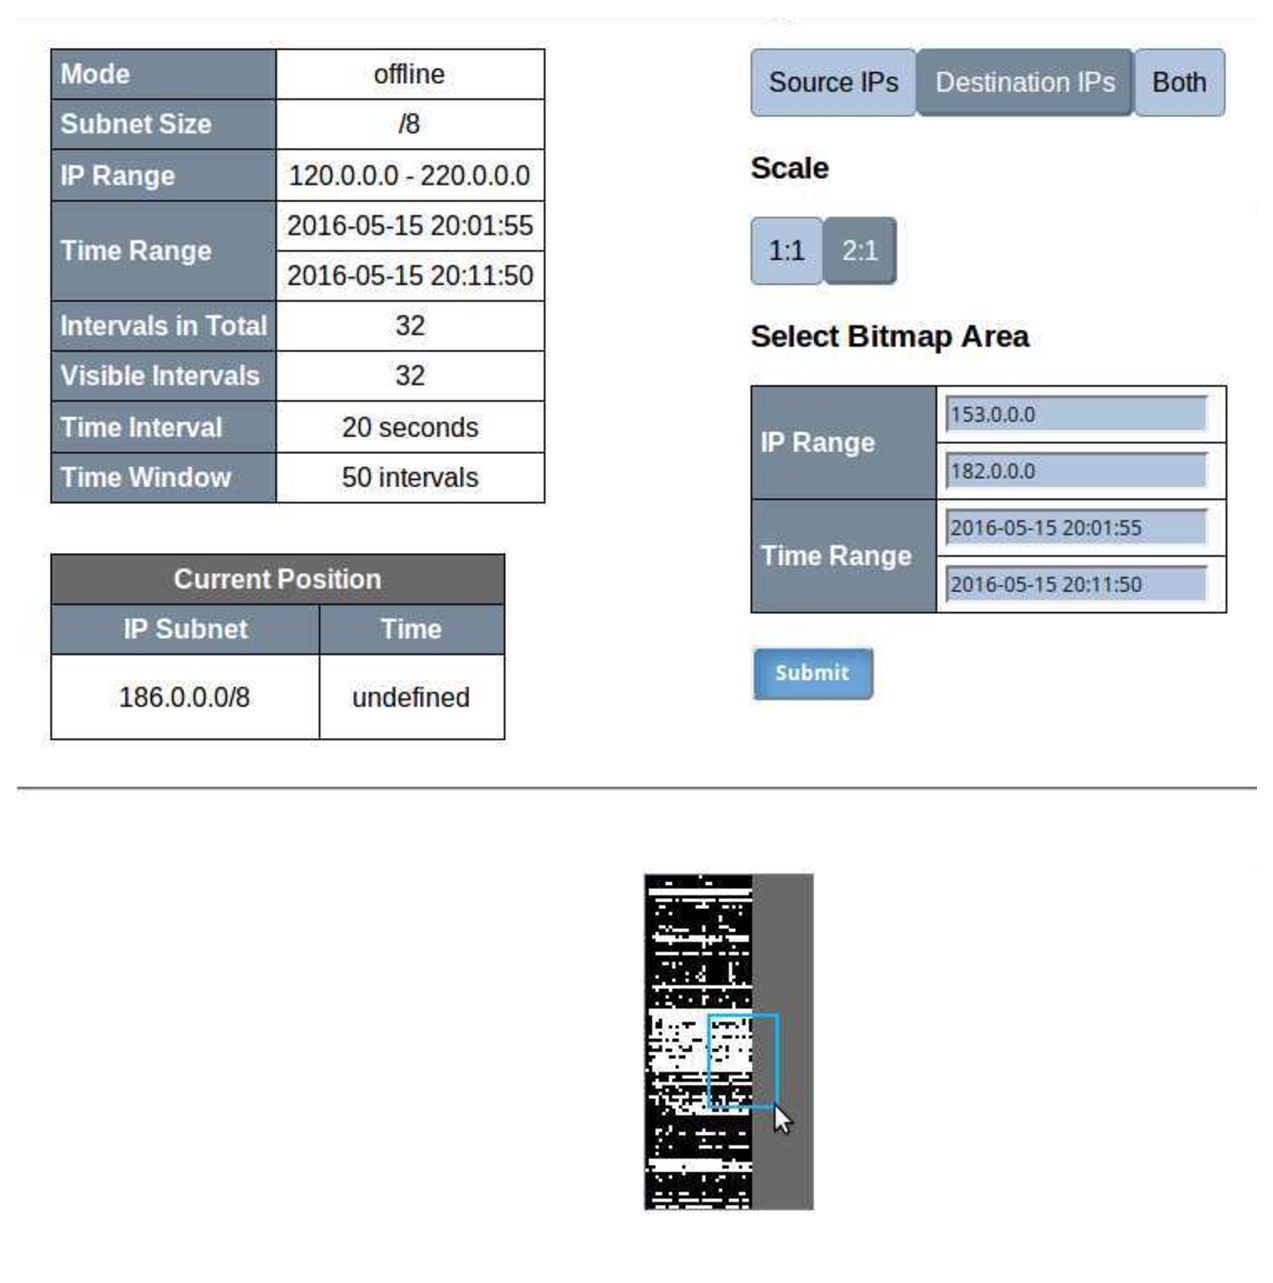
\includegraphics{fig/drag2}}} \hfill
      \caption{Selecting area by dragging cursor} \label{fig:drag1}
	\end{center}
\end{figure}

When the area is speficied, the form values of both ranges are updated with chosen limits values
(see Figure~\ref{fig:drag2}). The changed area is highlighted.
If one dimension value equals \textit{undefined}, maximum defined value
in that range is used. In case both values are \textit{undefined}, the full range
of both dimensions is inserted.

\begin{figure}[H]
   \begin{center}
		\scalebox{0.68}{\frame{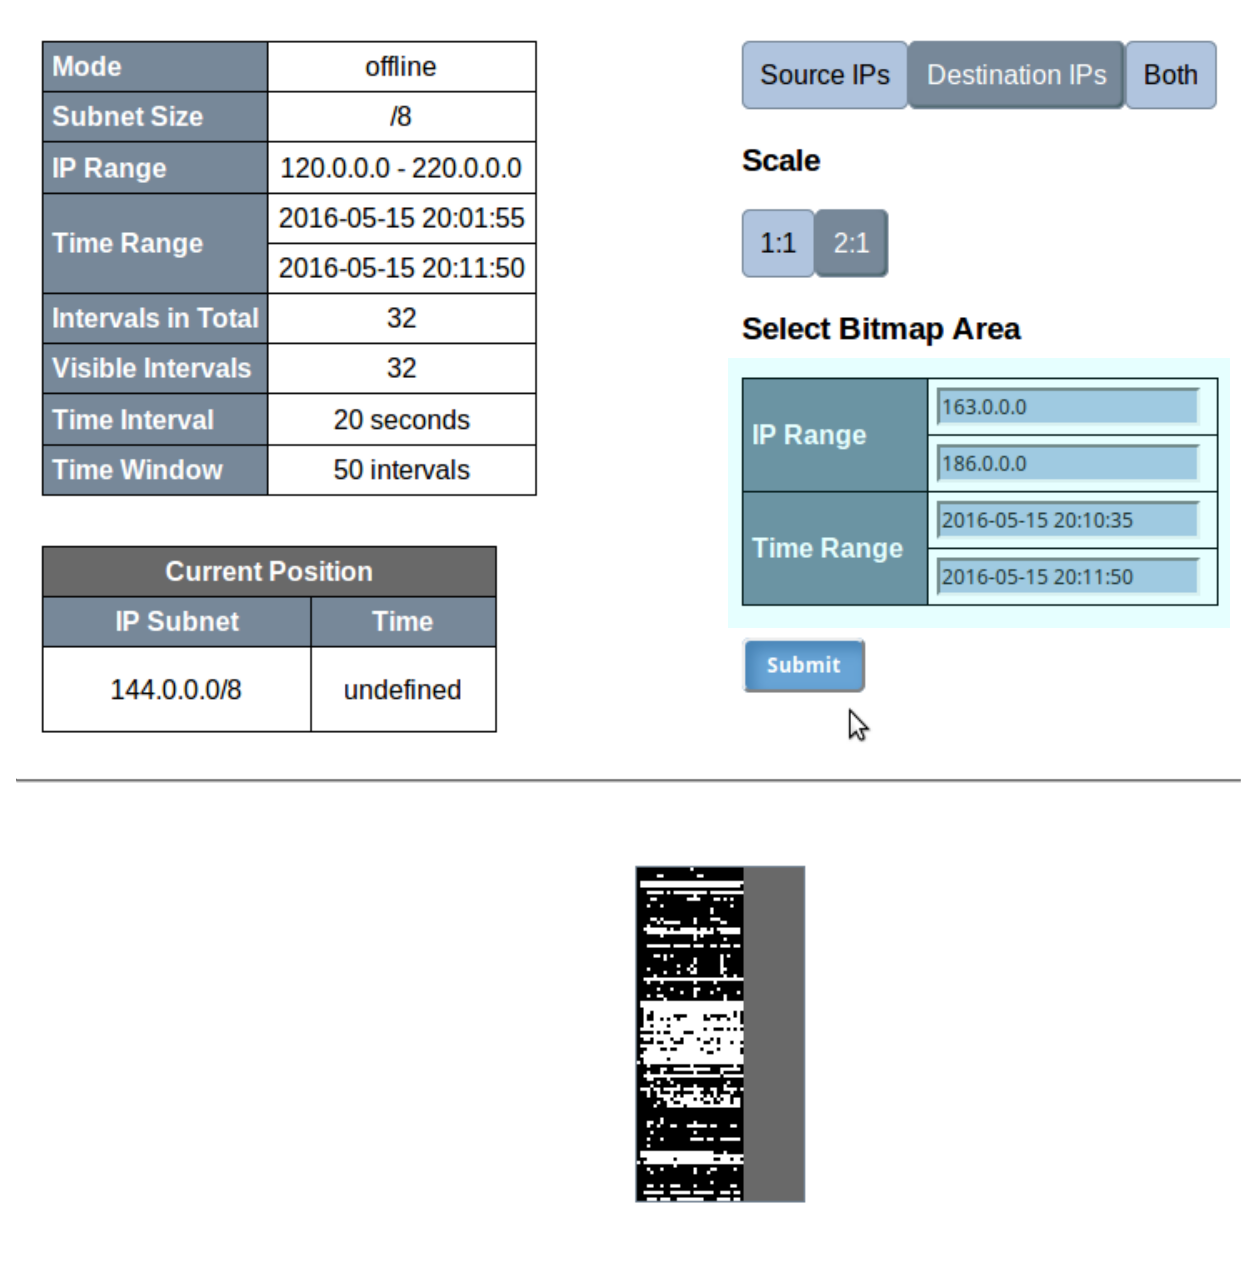
\includegraphics{fig/drag3}}} \hfill
      \caption{After releasing the cursor, form is updated} \label{fig:drag2}
	\end{center}
\end{figure}

After submitting the form, the \textbf{Selected Area} section is
displayed, containing specified area of the original image and its statistics
(see Figure~\ref{fig:drag3}). The form values specifying the selected
area are inserted in the characteristics.

\begin{figure}[H]
   \begin{center}
		\scalebox{0.75}{\frame{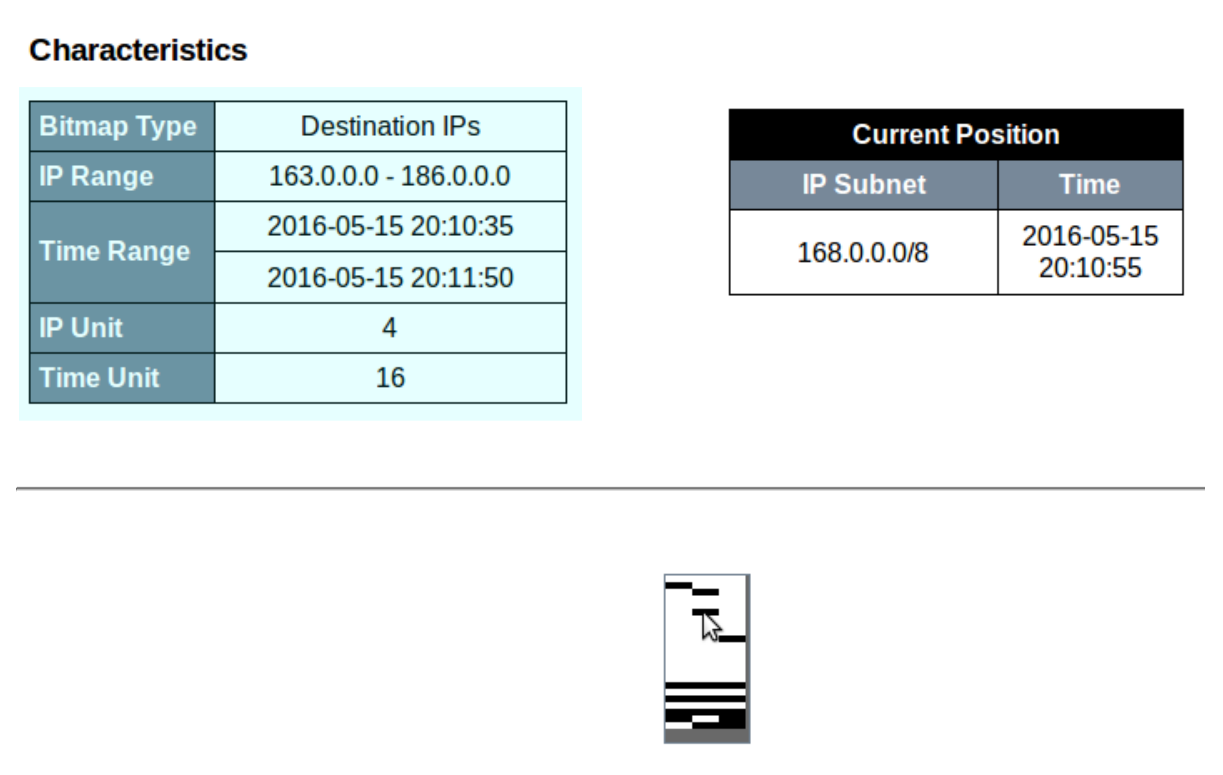
\includegraphics{fig/drag4}}} \hfill
      \caption{After submitting the form, Selected Area is displayed} \label{fig:drag3}
	\end{center}
\end{figure}

\subsubsection{Selected Area}
In the selected area, no modification options are available.
The left column is again dedicates to the \textbf{Characteristics}. This time,
only the attributes that are different from the main image are present.
Moreover, new attributes are added. Bitmap type defines from which storage
the area was created. IP and time interval units definine
the scaling of the image in both dimensions (for example, IP unit with value
$8$ means that activity of one subnet is displayed on 8 pixels on the $y$-axis).

Full list of displayed characteristics:

\begin{itemize}
   \item \itab{\footnotesize{Bitmap Type}} \tab{Mode the activity monitoring is in. Value: \textit{online} or \textit{offline}.}
   \item \itab{\footnotesize{IP Range}} \tab{Contains selected IP range. Value: \textit{<first IP> - <last IP>}}
   \item \itab{\footnotesize{Time Range}} \tab{Contains selected interval range as timestamps.}
   \item \itab{\footnotesize{IP Unit}} \tab{Defines scaling for subnets. One subnet is on \textit{<value>} pixels.}
   \item \itab{\footnotesize{Time Unit}} \tab{Defines scaling for intervals. One interval is on \textit{<value>} pixels.}
\end{itemize}

The right column contains \textbf{Current Position} which works analogically
to the top version. The two position indicators work independently.

The visualisation of the selected area below the characteristics only enables
the user to hover over, no additional selecting is available. 

\subsection{Client Interactivity}
In order to be able to change parts of the page dynamically without 
refreshing the main page, a~JavaScript file \textit{frontend.js} is included.
This script realises all the interaction with the web server and reacts
to server's responses. In this section, the main techniques
and event handlers are described.

Since the script uses the \textit{jQuery} library for easier element
access and modification, the script is not interpreted until the page is
fully loaded.

\subsubsection{Initialisation}
When the page is fully loaded, it contains all the characteristics
and default values from the server but the image initialisation is
up to the client.

If the user is currently in online mode, the top image is to be updated
periodically. Therefore, a~timeout handler is initialised with the
default value of 30\ seconds. The automatic update is implemented
in the function \texttt{auto\_update()}. The update cycle is started by
immediately calling the \texttt{update\_bitmap()} function. In the offline
mode, the image is updated only once at the beginning.

In addition to the image update, \textbf{Current Position} values and
form values are set to default (typically range limit values)
and all dynamic variables needed for the interactivity are set
(such as mouse index or IP version).

\subsubsection{HTTP Requests}
All \texttt{HTTP GET} requests and the corresponding reponses are handler by
function \texttt{http\_GET(\-url, callback, arguments, content\_type)} using
AJAX.

Upon calling this function, a~new request is created from passed \texttt{url} and
\texttt{arguments} creating the query. The \texttt{callback} function is set to
be called upon the server's response.


\subsubsection{Bitmap Update}
When the image is to be updated, the current version has to be obtained
from the server. This is done by \texttt{update\_bitmap()} function which
sends a~HTTP GET request to the server, using the \texttt{http\_GET} handler
and as a~callback function, \texttt{set\_bitmap()} is passed to the handler.

When the response is received, the callback function checks if the requested
bitmap was available. If yes, it creates a new \texttt{<img>} element in
designated block element with ID \texttt{bitmap\_inner}, containing the
server's encoded response.

In addition to displaying the image, the server also sends new statistics
values in the response header. Thanks to this, the client can keep
the user up to date with the total number of intervals and the
time range of the displayed activity in online mode.

\subsubsection{Form Submit}
When submitting the form, the usual action would be sending the values
as a~query to the server and reloading the page. Here, if the page
were reloaded, it would lose all the data from the last session, such as
last visited position. In order to avoid this, a~custom handler is
implemented for click event for \texttt{submit} class elements.

This handler disables the default action, parses and validates
the form values by comparing the selected range limits to the
full bitmap limits.

Because JavaScript does not have any convenient
comparison function for IP addresses, a~custom function
\texttt{compare\_ips(first\_ip, last\_ip)} is used. If reduced IPv6 addresses
are entered, they are normalized at first. Then, the two addresses are
split into parts based on the delimiter (\quotes{.} in IPv4 and \quotes{:} in IPv6) and
each part is compared separately.

After arguments validation, an~HTTP GET request is created. Upon the
server's response, a~callback function \texttt{set\_selected\_area()} is called.
Here, the Selected Area section is set to \texttt{visible},
the area characteristics is inserted into designated elements and the
current position is initialised to default values.

\subsubsection{Current Position Update}
When hovering over the activity visualising images, a~custom \texttt{mousemove}
handler is implemented. It calculates the cursor position relatively to the
image top left corner and substracts the size of the image border.

Subsequently, it sends a~request to the server to get the current position
values, providing the underlying image (original or selected area),
first values in range and the current ones in the query.

When the server returns the current values, The corresponding
\textbf{Current Position} section is updated and the element
background is set based on the activity status.

\subsubsection{Interactive Area Select}
In order to spare the user from having to read the limit ranges of their
specified area and insert them to the form manually, there is a~better
option available. The user can drag the mouse over the area they want
to examine and the values are automatically inserted in the form.

This functionality uses the current position indicator for converting
the indices to IP and time values. To implement this functionality,
three event handlers must be implemented --
\texttt{mousedown} initialising the drag, \texttt{mousemove} and
\texttt{mouseup} finishing the drag and updating the form values.

During the \texttt{mousedown} event, the current position is saved and a~block
element of a~distinctive colour is made visible for the user to know
which area they have chosen so far.

This event is followed by \texttt{mousemove}, where the block over the area
is changed to adjust the user's selection.

Finally, \texttt{mouseup} event is registered. To enable choosing
the edge positions, the \texttt{mouseup} can be carried out anywhere
on the page but only if the drag flag is active, the handler is activated.
In this handler, the values are inserted in the form un such order that
they respect the left-to-right, top-to-bottom orientation. By doing so,
the user has more flexibility when creating the area and can move the
mouse in all directions.

Additionally, the area selection enables the user to use the \textit{undefined}
areas. When only one of the two dimension values is undefined, the maximum
defined value is taken. By using this principle, the user does not need to
worry about dragging the cursor too far and can use this functionality to
display the whole interval for a~choosen subnet  when the current number
of visualised intervals is too small for accurate in-place selection.

\csdoublequotesoff

% Testing
\chapter{Testing}\label{sec:chapter5}
During the system development, the repeated manual testing of all the main parts
of the system was required (the backend, web server and the web client).
However thorough, the manual testing is not sufficient for being the
only way of testing the system that is under development and frequently changed.

In order to test the most crucial and frequent operations on various data,
unit tests were created. These tests are possible due to the system's modularity.
However, they do not cover everything, only the parts
of the functionality that can be isolated. These tests can be found in
the source code attached to this thesis.

User testing is required to test the rest of the functionality.
The system was introduced to the consultant and the supervisor and their
feedback was taken into account and helped to improve some of the
principles and the user interface.
This remains an ongoing process as more users start using this system and
more feedback is expected in the future.

\section{Manual Testing}
Since the system contains custom data storage and all its parts are
interacting with each other, the development of the application started
with the backend which is responsible for monitoring and storing the activity
to ensure the validity of the storage data. The development continued
with the server retrieving and manipulating the stored data to make
sure that the data is read and visualised correctly. This was soon followed
by the interactive frontend where it had been ensured that the activity
characteristics and the images were displayed correctly and the user was given
valid information when interacting with the interface.

Manual testing of the backend and the server was
realized using the standard and error console output, using debug messages.
When debugging the frontend, the most efficient way to test it during the
running time was to write the required status updates in the browser console log.

\section{Unit Tests}
In addition to the manual testing, unit tests were written for the backend
and the server. These use the functionality from the backend accessible from
backend header file \textit{ip\_activity.hpp} and the visualisation handler
in \textit{activity\_visualisation.py}.

They test various input parameter combinations, and more importantly, check
if the bitmap in the backend that is stored in the binary storage equals
the bitmap retrieved by the server and manipulation with the bitmap
on the server.

Backend parameters testing can be found in \textit{backend\_tests.sh}
and server parameters testing in \textit{server\_tests.sh}. Testing
the storage content is in \textit{bitmap\_tests.sh} and in case of failure,
offers an output showing the differences. Configuration file testing
can be found in \textit{config\_tests.sh} and it tests the backend's
creation and server's loading of the configuration file.
In order to enable running all tests, \textit{run\_tests.sh} was created.

All tests can be run with a~verbose parameter \texttt{-v} which displays
error message in case of failure. It also prints configuration file
content and binary storage content for better demonstration. In case
of bitmap tests, the results differ due to bitmap transposition by the
server.

The functionality of the server based on the incoming requests is not
suited for unit testing as it should not be standalone and not based
on networking.

\section{User Testing}
This type of testing was realized in several rounds. The participants
were introduced to the main principles and the frontend and asked to suggest
improvements.

\subsection{The Backend and the Web Server}
In the first round, the main goal was to find out if the data processing
and storage maintenance principles were sufficient.

The following suggestions were made:

\begin{enumerate}
   \item The system should not be based on \texttt{SIGALRM} due to offline
   mode where the flows are processed in one go. The field \texttt{TIME\_FIRST}
   should be used for this instead.
   \item The code should be more structuralized in order to be able to
   call the storage functions separately and test them without having to
   start the system.
   \item The server should obtain the beginning of the oldest visible interval
   after each bitmap update in addition to the passed number of intervals so that
   in the online mode, this value can be displayed to the user.
\end{enumerate}

Based on the feedback, the folowwing improvements were made:

\begin{enumerate}
   \item In both offline and online mode, the system filters the traffic
   based on the \texttt{TIME\_FIRST} of the flow. This value is also used
   for finding out if the current flow belongs to the current interval or not which
   enables older flows to be stashed and inactivity to be shown when skipping multiple
   intervals. The configuration file has a different structure for each mode
   so that the server can distinguish them.
   \item In order to make unit testing possible, the backend header file
   and a~new server module were created, which was dedicated solely
   to manipulate with the bitmap and its characteristics.
   \item After each interval, the configuration file is updated and the
   oldest interval's \texttt{TIME\_\-FIRST} is stored, along with the total
   number of intervals.
\end{enumerate}

\subsection{Web Client}
In the second round, the aim was to test the frontend and find out what
information the user wants to see directly on the page and what the image
should look like. The feedback was as follows:

\begin{enumerate}
   \item The 1:1 ratio is not enough for the user to distinguish small
   areas of a few pixels.
   \item Since the image includes only passed intervals, the user does
   not have such a~clear idea about the full size of the image and the
   proportions when the intervals shown have not reached the time window.
   \item The selected area should be scalable based on which dimension
   the user wants to examine more in detail.
   \item The URL does not change based on the requests made which does not
   allow the user to use the URL to access a specific data. This could be
   a~useful improvement.
   
\end{enumerate}

The feedback was evaluated and the following improvements were made to the system:

\begin{enumerate}
   \item The original bitmap has now the option of being displayed in
   2:1 ratio. The scaling functionality is implemented for any X:1 ratio
   so that custom ratios can be added in the future.
   \item The images always keep the full proportions. An \textit{undefined}
   value is added so that when the user displays the image with a smaller
   number of intervals, the rest of the image has a distinctive appearance
   to show that the activity has yet to be determined.
   \item The selected area also retains the size and proportions of the original
   image. In order to enable the user to focus on a~specific dimension, the
   principle of selecting area scales both dimensions maximally, but does not
   allow the full size to be exceeded. By using this technique, the smaller the size
   of the dimension selected, the more it is scaled.
   \item Since this suggestion does not address a~crucial functionality,
   it does not have such a~high priority. However, this improvement could
   indeed extend the possible ways of interacting with the frontend so this
   functionality is intended to be added in the future.
\end{enumerate}

% Results
\section{Results}\label{sec:results}
The main purposes of this thesis are to reduce storage size needed for
storing data containing IP address activity and by doing so, reduce
time needed for data lookup in a~bigger volume of data using gained information
about the activity.
In the folowing sections, the performance, storage and lookup time comparison will be discussed.

\subsection{Performance}
The throughput of a~probe during the peak hours equals 160 000 flows per second.
In the developed system, the backend is able to process up to 550 000 flows
per second in the offline mode. Therefore it has no problems with
30 000 flows per second measured during average traffic hours.

\subsection{Storage Size Comparison}\label{sec:storage_cmp}
In order to compare storage size, let us assume the following parameters:

\begin{itemize}
   \item The target address space is a~/16 subnet of IPv4 addresses.
   \item The granularity equals /32 (individual addresses).
   \item The interval length is 5~minutes.
   \item The time during which the activity is to be mmonitored is one day.
\end{itemize}

In the case of unoptimized storage, stored flow records that were captured by
10 probes during one day have the total size of 200 GB.

When using the developed system, the size of the storage space is as follows:
\begin{align*}
   &address\_space = \frac{2^{16}}{2^{32-0}} = 2^{16} \mbox{ addresses} \\
   &interval\_length = 300 \mbox{ seconds}\\
   &seconds\_in\_day = 86400 \\
   &time\_window = \frac{seconds\_in\_day}{interval\_length} = \frac{86400}{300} = 288 \mbox{ intervals}\\
   \\
   &storage\_size = CEIL(\frac{address\_space}{8}) \cdot time\_window \mbox{ B}\\
   &storage\_size = CEIL(\frac{2^{16}}{2^3}) \cdot 288 = 2^{13} \cdot 288 = 8192 \cdot 288 \mbox{ B}\\
   &storage\_size = 2,359,296 \mbox{ B} \approx 2359.30 \mbox{ kB} \approx 2.36 \mbox{MB}
\end{align*}

Since the system stores information about three types of addresses, the total size
of stored data would three times this size, or:

\begin{equation}
   2,359,296 \cdot 3 = 7,077,888 \mbox{ B} \approx 7.08 \mbox{ MB}
\end{equation} 

The difference between the storage containing flow records and solely
IP activity is then defined as follows:
\begin{equation}
\frac{7,077,888}{200\cdot10^{9}} \cdot 100\% = \frac{1728}{48,828,125} \cdot 100\% \approx \frac{1}{28257} \cdot 100\% \approx 0.0035\%
\end{equation}

From the result can be concluded that the developed system uses in this case
$28257\times$ less storage space than the ordinary system. If the system
were to maintain 200\ GB of data using the same parameters, it would contain activity
during 28 257 days which is approximately 77 years.

The only data that is not used for storing activity in this system are the padding bits
rounding up the row size to the nearest Byte. This matter is discussed in
more detail in Section~\ref{sec:bitmap_storage}.

\subsection{Lookup Time Comparison}
Assuming the data parameters from the storage comparison in Section~\ref{sec:storage_cmp},
even with no indexing involved, generally speaking, going through 200 GB data takes much more time
than going through mere $2.3$ MB.

When using \textit{nfdump} to process the unoptimised storage, going through
the whole storage in order to analyse activity of one IP address during the
whole time period (one day) took 40 minutes. As \textit{nfdump} did not
have any information on the flows, it had to search all present flow records, one by one.

In this system, querying data in the used binary storage is much more effective.
In order to get an index for a~particular IP address or interval,
easy calculation is executed by the server (discussed in Section~\ref{sec:indexing_principles})
and as a result, offsets of both dimensions are obtained.

So, in order to find out IP activity for one day, the index of the address
is obtained based on the first address in range, address granularity and
the wanted address. After having the offset, only \texttt{<number of intervals>}
values are analysed. When processing by the server, it transposes the dimensions
and shifts the storage by the offset of the beginning, so that activity of
one address is in one row in chronological order. As a result, user can
determine the active intervals easily.

\csdoublequotesoff

% Conclusion
\chapter{Conclusion}\label{sec:chapter6}
The volume of flow records transmitted through the network is growing.
In order to be able to query data faster, an effective way of storing
the data and indexing them is required. This thesis addresses this problem
and particularly focuses on storing and visualising activity of
communicating IP addresses. The IP activity can be defined by a~binary
value which reduces the total size of the storage.

The aim of this thesis was to develop a~system that monitors, stores and 
visualises IP activity. This system contains a~backend, a~NEMEA module,
which scans incoming traffic and stores the relevant activity to binary storage
and its characteristics to a~configuration file. The fact that this storage
only uses one bit to represent activity of one subnet during one interval
effectively reduces the the lookup time.

The stored data is then used by the web server to provide the visualised
form of the activity and its characteristics to the user via a~web interface.
The server uses a~separate module for bitmap manipulation and data gathering.

When comparing the results with \textit{nfdump} tool in Section~\ref{sec:results},
it was established that the developed system enables storing IP activity
in a~more effective way than it is currently done -- together with other attributes
contained in the flow records. The significantly reduced storage size and easily
performed indexing also make querying data much faster than by analysing all records
one by one and offers a way of visualising the activity to the user in a~comprehensive manner.

Additionally, the system enables the user to display areas of interest in more
detail. The gained activity information can then be used to narrow the amount
of data processed in other networking tools, such as NfSen.

Currently, the system is in a~state that is usable but not final.
As this system is deployed and used by various types of users, new
requirements for the system can be obtained.
The currently planned improvements include to:

\begin{enumerate}
   \item Integrate the results of this work with NfSen, with
   distributed collector and fdistdump \cite{fdistdump}.
   \item Enable the user to interact with the server not only via the web
   interface, but also by sending queries directly from the browser.
   \item Add a~system for applying custom ratios to both images (the original
   and the selected area).
\end{enumerate}

%=========================================================================
 % viz. obsah.tex

  % Pouzita literatura
  % ----------------------------------------------
\ifslovak
  \makeatletter
  \def\@openbib@code{\addcontentsline{toc}{chapter}{Literatúra}}
  \makeatother
  \bibliographystyle{czechiso}
\else
  \ifczech
    \makeatletter
    \def\@openbib@code{\addcontentsline{toc}{chapter}{Literatura}}
    \makeatother
    \bibliographystyle{czechiso}
  \else 
    \makeatletter
    \def\@openbib@code{\addcontentsline{toc}{chapter}{Bibliography}}
    \makeatother
    \bibliographystyle{plain}
  %  \bibliographystyle{alpha}
  \fi
\fi
  \begin{flushleft}
  \bibliography{literatura} % viz. literatura.bib
  \end{flushleft}

  % Prilohy
  % ---------------------------------------------
  \appendix
\ifczech
  \renewcommand{\appendixpagename}{Přílohy}
  \renewcommand{\appendixtocname}{Přílohy}
  \renewcommand{\appendixname}{Příloha}
\fi
\ifslovak
  \renewcommand{\appendixpagename}{Prílohy}
  \renewcommand{\appendixtocname}{Prílohy}
  \renewcommand{\appendixname}{Príloha}
\fi
  \appendixpage

\ifslovak
  \section*{Zoznam príloh}
  \addcontentsline{toc}{section}{Zoznam príloh}
\else
  \ifczech
    \section*{Seznam příloh}
    \addcontentsline{toc}{section}{Seznam příloh}
  \else
    \section*{List of Appendices}
    \addcontentsline{toc}{section}{List of Appendices}
  \fi
\fi
  \startcontents[chapters]
  \printcontents[chapters]{l}{0}{\setcounter{tocdepth}{2}}
  %=========================================================================
% (c) Kateřina Pilátová, 3BIT
\setlength{\parindent}{0em}
\setlength{\parskip}{1em}

\csdoublequotesoff
\chapter{CD Content}
This section is concerned with the contents of the attached CD.
It includes the basic set of files forming the developed system.

However, not all files needed for running the system are included -- the
autotool configuration file and IP address library for C++ which was
extended for the purposes of this thesis are available in the git
repository forks (see Section~\ref{sec:requirements}).

The main sections are:
\begin{itemize}
  \item \itab{\footnotesize{\texttt{.}}} \tab{The root directory contains source files, scripts and guides.}
  \item \itab{\footnotesize{\texttt{images/}}} \tab{In this directory, visualised images are to be stored.}
  \item \itab{\footnotesize{\texttt{tests/}}} \tab{This directory is dedicated to testing and contains test suite.}
  \item \itab{\footnotesize{\texttt{doc/}}} \tab{Here the the source files for the thesis text version are located.}
\end{itemize}

Even though most of the files contain a~section with the used~licence, \textit{licence.txt} file is also included.


\chapter{Installation Guide}
\section{Requirements}\label{sec:requirements}
In order to use the system, the following requirements must be met:
\begin{itemize}
   \item The target system must have g++ installed.
   \item The target system must have Python 2 or 3 available.
   \item In order to run the web client, the target browser must have JavaScript enabled.
   \item In order to install the backend, access to Nemea repository is required.
   \item It is essential to download the updates of the Nemea repository and Nemea framework
   from my forked repository of Nemea-Framework~\cite{my_repo_framework} and Nemea-Modules~\cite{my_repo_modules}.
   In there, changes of autotools configuration file and \textit{ipaddr\_cpp.h} are up-to-date.
\end{itemize}

\section{Additional Packages}
\begin{itemize}
   \item For backend, only C++ \textit{Boost} library and \textit{yaml-cpp} version 0.5.3 libraries are required.
   In order to run the backend on a~machine (for example \textit{benefizio}) where the 0.5.3 version is not available,
   the library has to be installed straight from the source~\cite{yaml_cpp} and the path to it included in the
   \textit{Makefile.am}.
   \item The attached archive contains a~script \textit{install\_dependencies.sh} which should
   install the required packages for both C++ (if the 0.5.3 version is available) and Python both 2.x and 3.x.
\end{itemize}

\section{Running the System}
The backend has to be run first so that it can create the bitmaps and more importantly, the configuration file.
The backend parameters are discussed in Section~\ref{sec:backend_params} and can be displayed by
entering \texttt{-h [trap]} parameter.

The server program cannot be executed until the configuration file is created. Server's parameters
are listed in Section~\ref{sec:server_params} or can be displayed by entering \texttt{-h} or \texttt{-{}-help}
parameter. When executing the server, make sure to set up the port based on your options.

The frontend program has to run in a browser which has \textit{JavaScript} enabled. It does not need
an internet connection as the \textit{jQuery} library is provided in the archive.
 % viz. prilohy.tex
\end{document}
